\chapter{Signal Modeling}\label{sig_model}

The shape of the reconstructed signal mass is extracted from the bulk graviton and $W'$ samples to model the peak of the resonance. The natural width of the resonance is considered to be  sufficiently small to be neglected when compared to the detector resolution. In the final analysis of the $M_{VZ}^{T}$ spectrum, the discovery potential and the exclusion power depend both on an accurate description of the signal shape. We adopt an analytical description of the signal shape, choosing a single Crystal-Ball function (i.e. a Gaussian
core with power-law low-end tail) to describe the CMS detector resolution. The typical
width of the Gaussian core is about 5$\%$-7$\%$ of the nominal mass. The analytical description
of the signal shape allows us to probe mass points for which there is no generated sample by
interpolating the shape parameter. No appreciable differences have been observed
in the $M_{VZ}^{T}$ signal shape between the low-purity and the high-purity categories.
Table \ref{tab:Bulksignal} and table \ref{tab:Wprimesignals} show the mass points and the fit range for each signal hypothesis. The transverse mass fits in the signal sample are shown in the figures \ref{fig:fits6a},\ref{fig:fits6b}, and \ref{fig:fits7}. Figure \ref{fig:fits9} shows the simulated $M_{VZ}^{T}$ distribution for resonance masses from 800 to 2000 GeV after the interpolation process. The different distributions are normalized to the corresponding efficiencies.

\begin{table}[h]
\begin{center}
\caption{Different mass points to fit the signal shape for Bulk graviton model.}
\label{tab:Bulksignal}
\begin{tabular}{ccc} \hline
Mass point (GeV) & Mean (GeV) &  Fit window (GeV) \\ \hline
800 & 763 & [620,900] \\
1000 & 930 & [670,1190] \\
1200 & 1100 & [720,1424] \\
1400 & 1283 & [850,1657] \\
1600 & 1461 & [1035, 1887] \\
1800 & 1640 & [1168, 2112] \\
2000 & 1819 & [1295, 2342]
\end{tabular}
\end{center}
\end{table}

\begin{table}[h]
\begin{center}
\caption{Different mass points to fit the signal shape for W prime model.}
\label{tab:Wprimesignals}
\begin{tabular}{ccc} \hline
Mass point (GeV) & Mean (GeV) &  Fit window (GeV) \\ \hline
800 & 760 & [600,1000] \\
1200 & 1092 & [560,1500] \\
2000 & 1685 & [700, 2100]\\
\end{tabular}
\end{center}
\end{table}

\begin{figure}[!ht]
\caption{ Fit of the Bulk Graviton signal samples for different mass points in the HP category.}
\begin{tabular}{cc}
  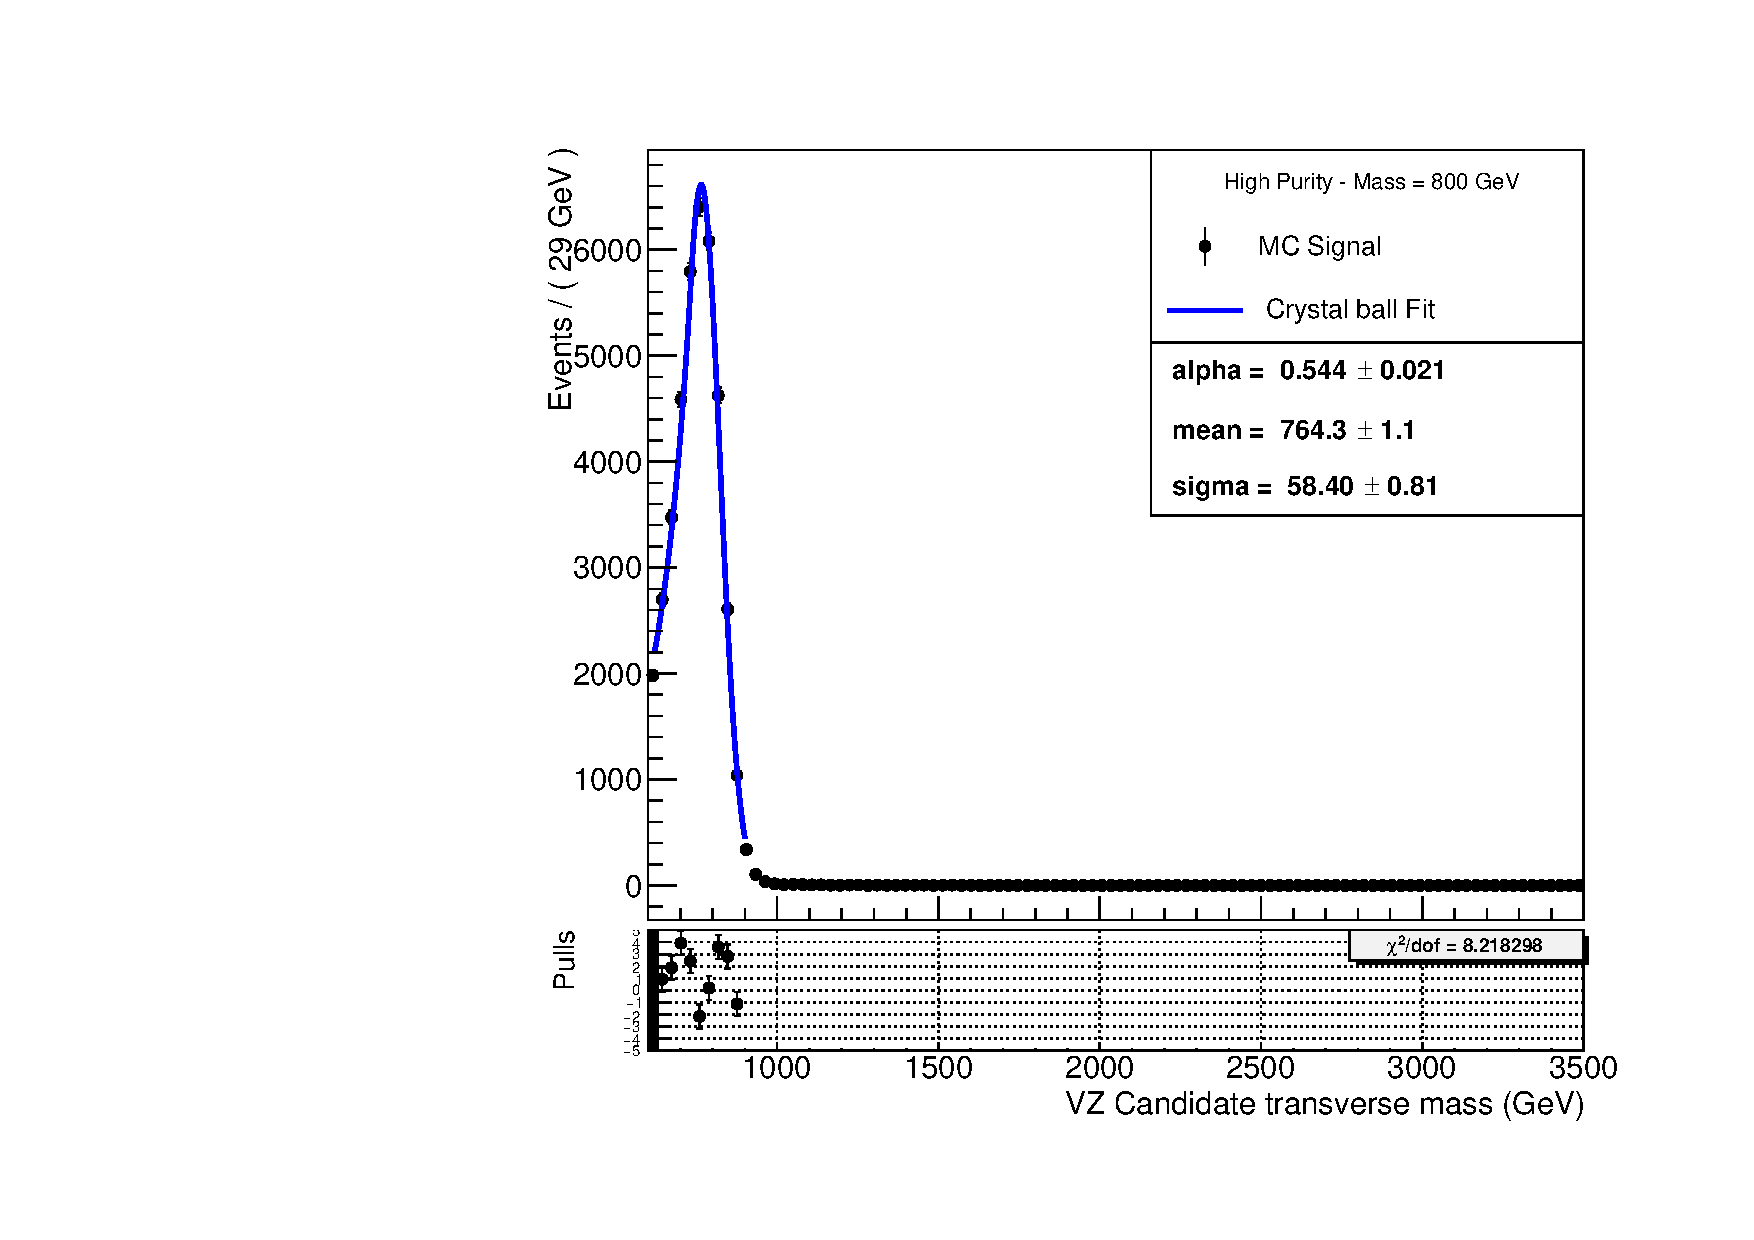
\includegraphics[width=170pt]{figuresARC/fits/BulkGravHP800.pdf} &
  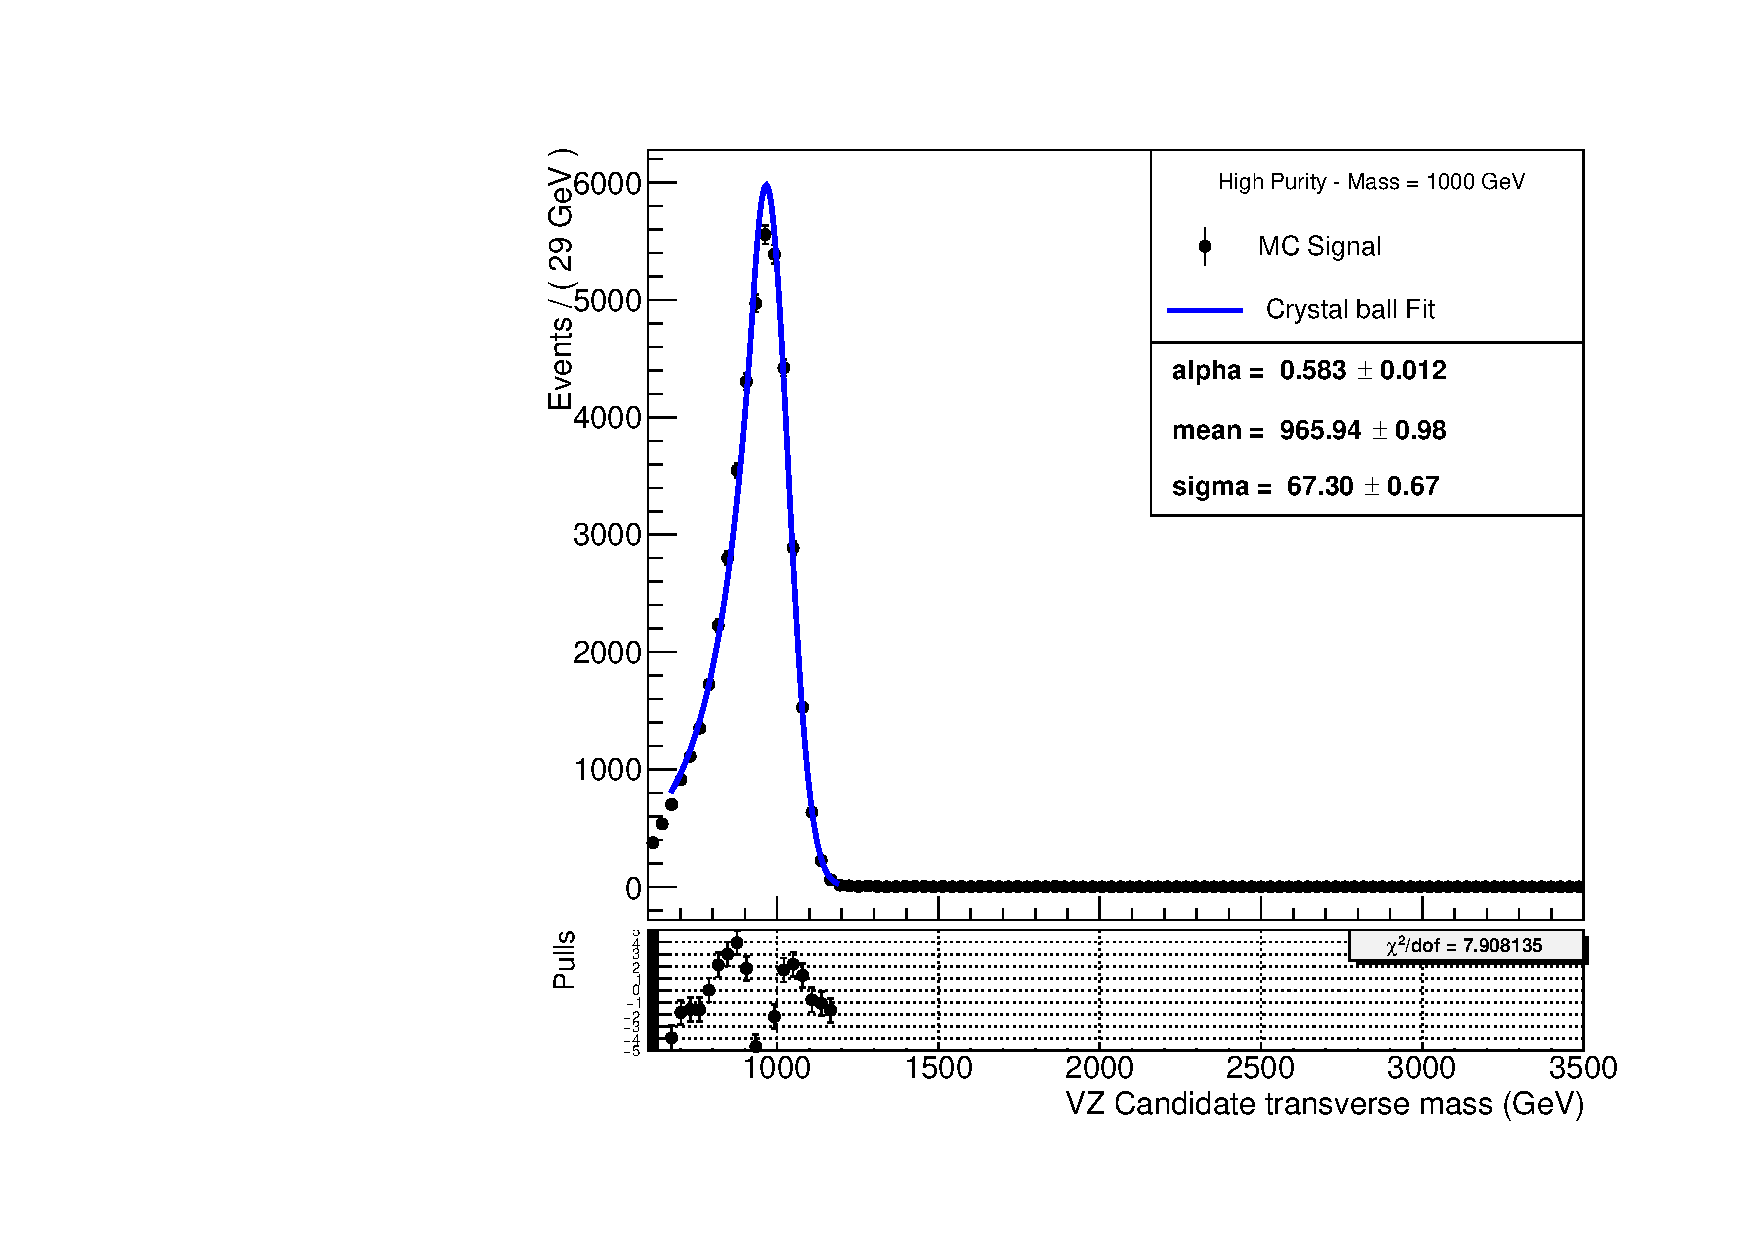
\includegraphics[width=170pt]{figuresARC/fits/BulkGravHP1000.pdf}\\
  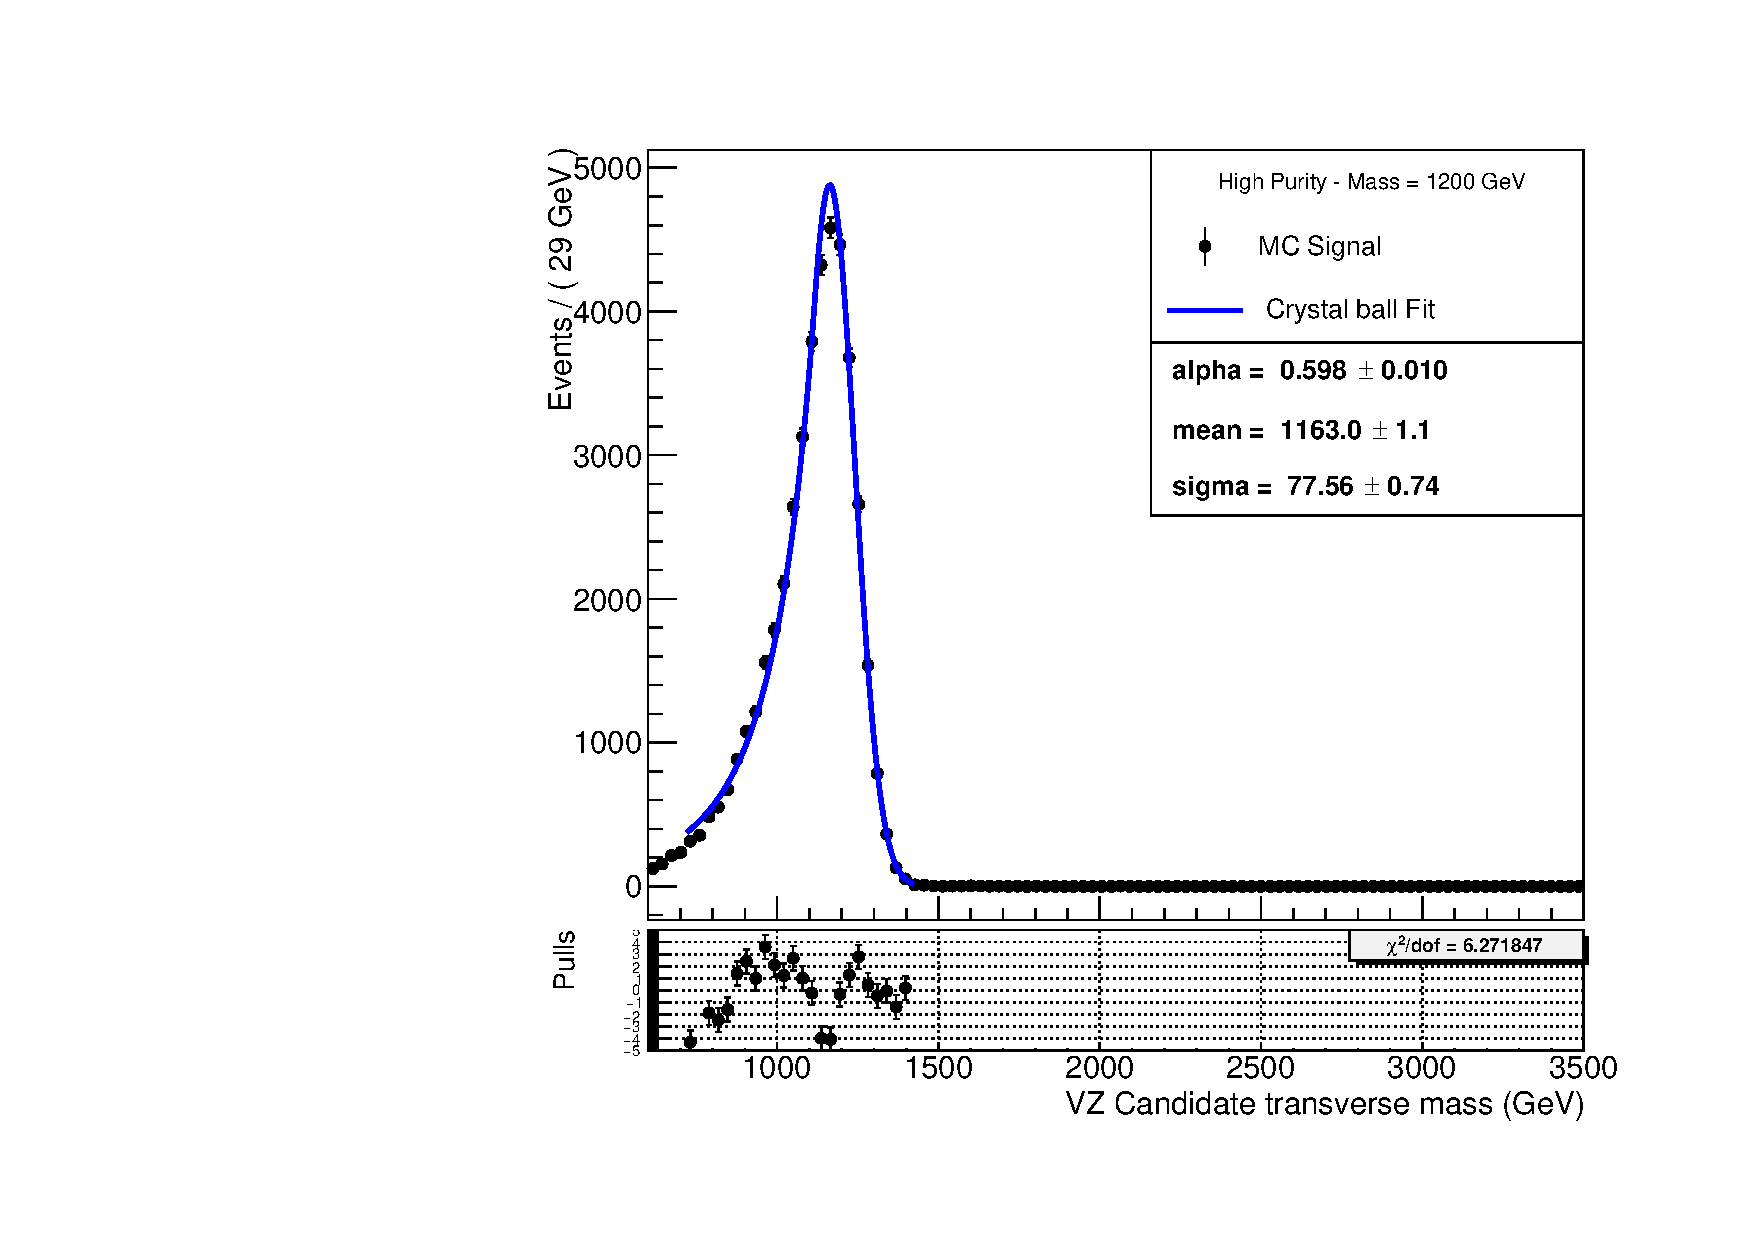
\includegraphics[width=170pt]{figuresARC/fits/BulkGravHP1200.pdf} &
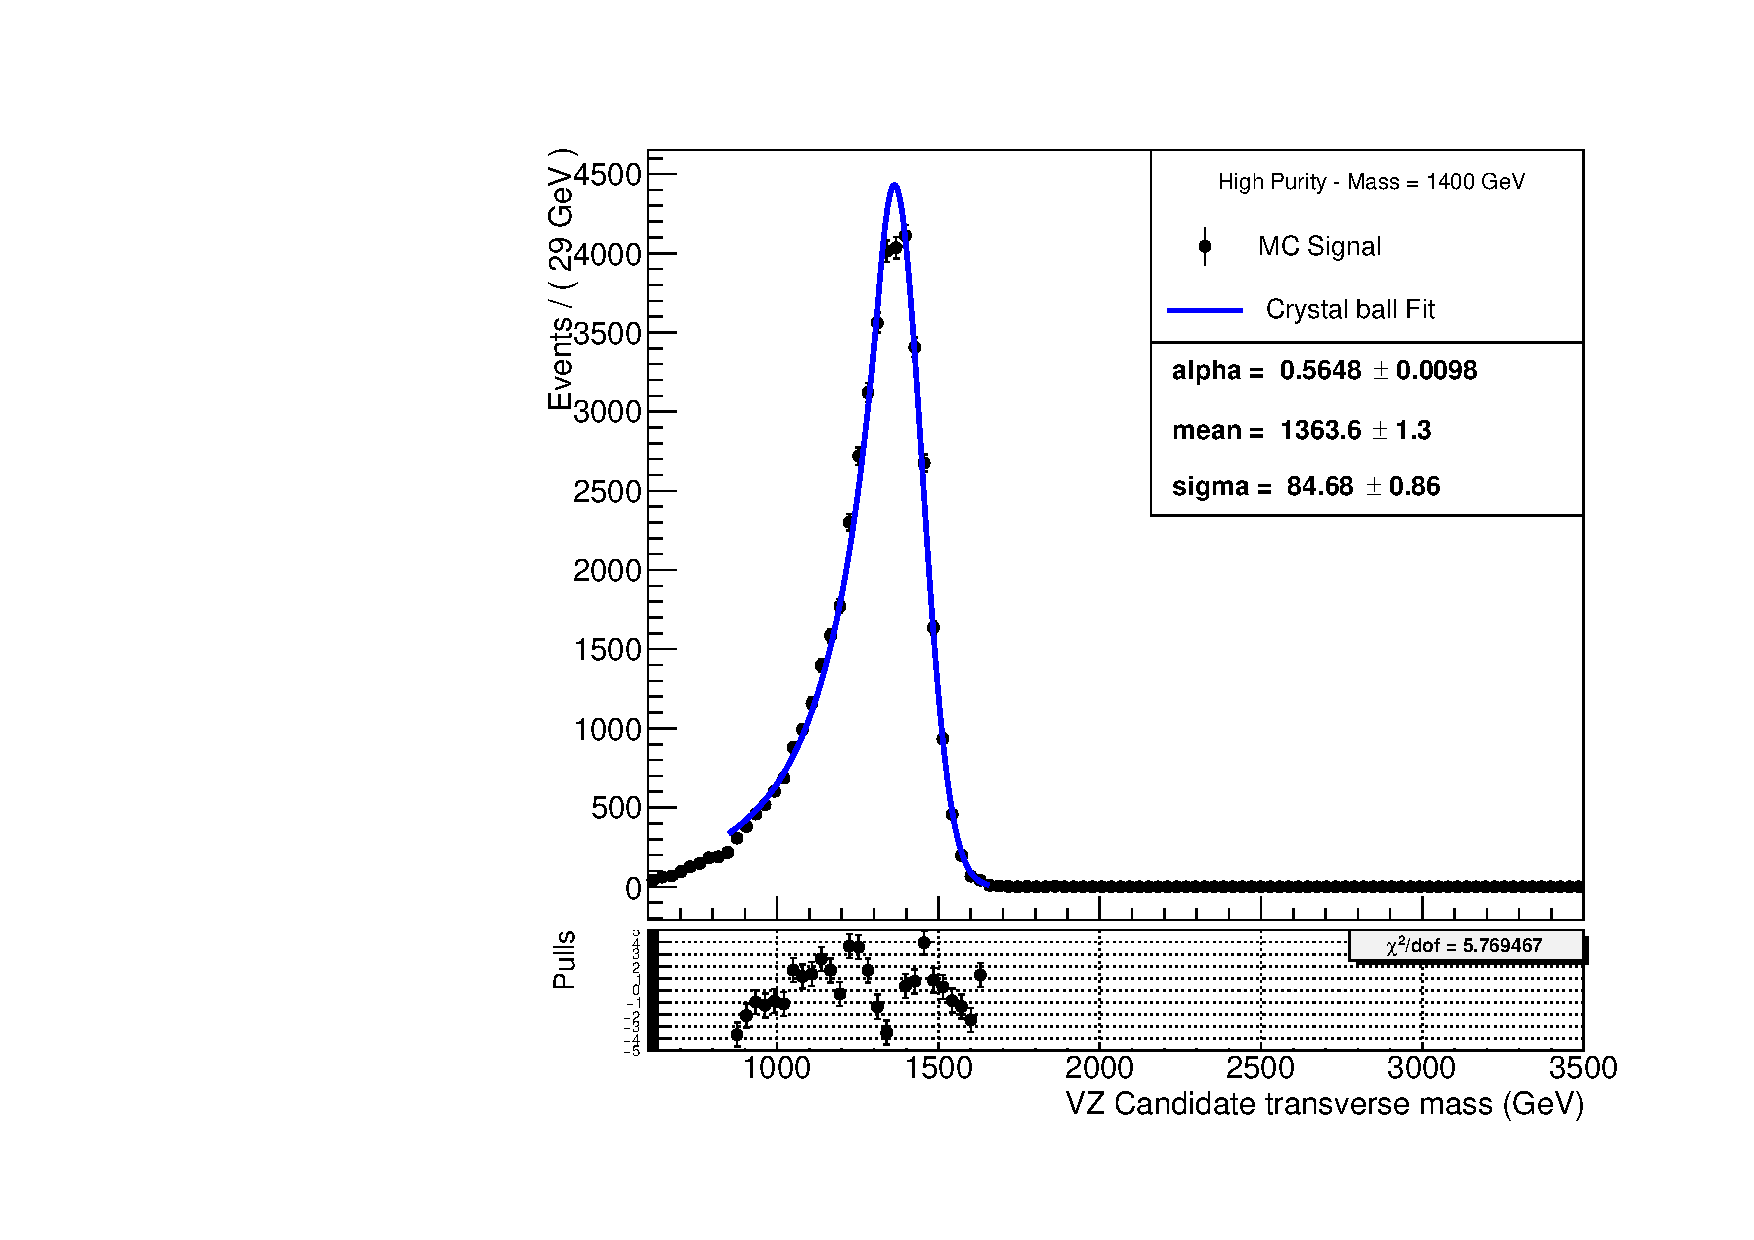
\includegraphics[width=170pt]{figuresARC/fits/BulkGravHP1400.pdf}  \\
  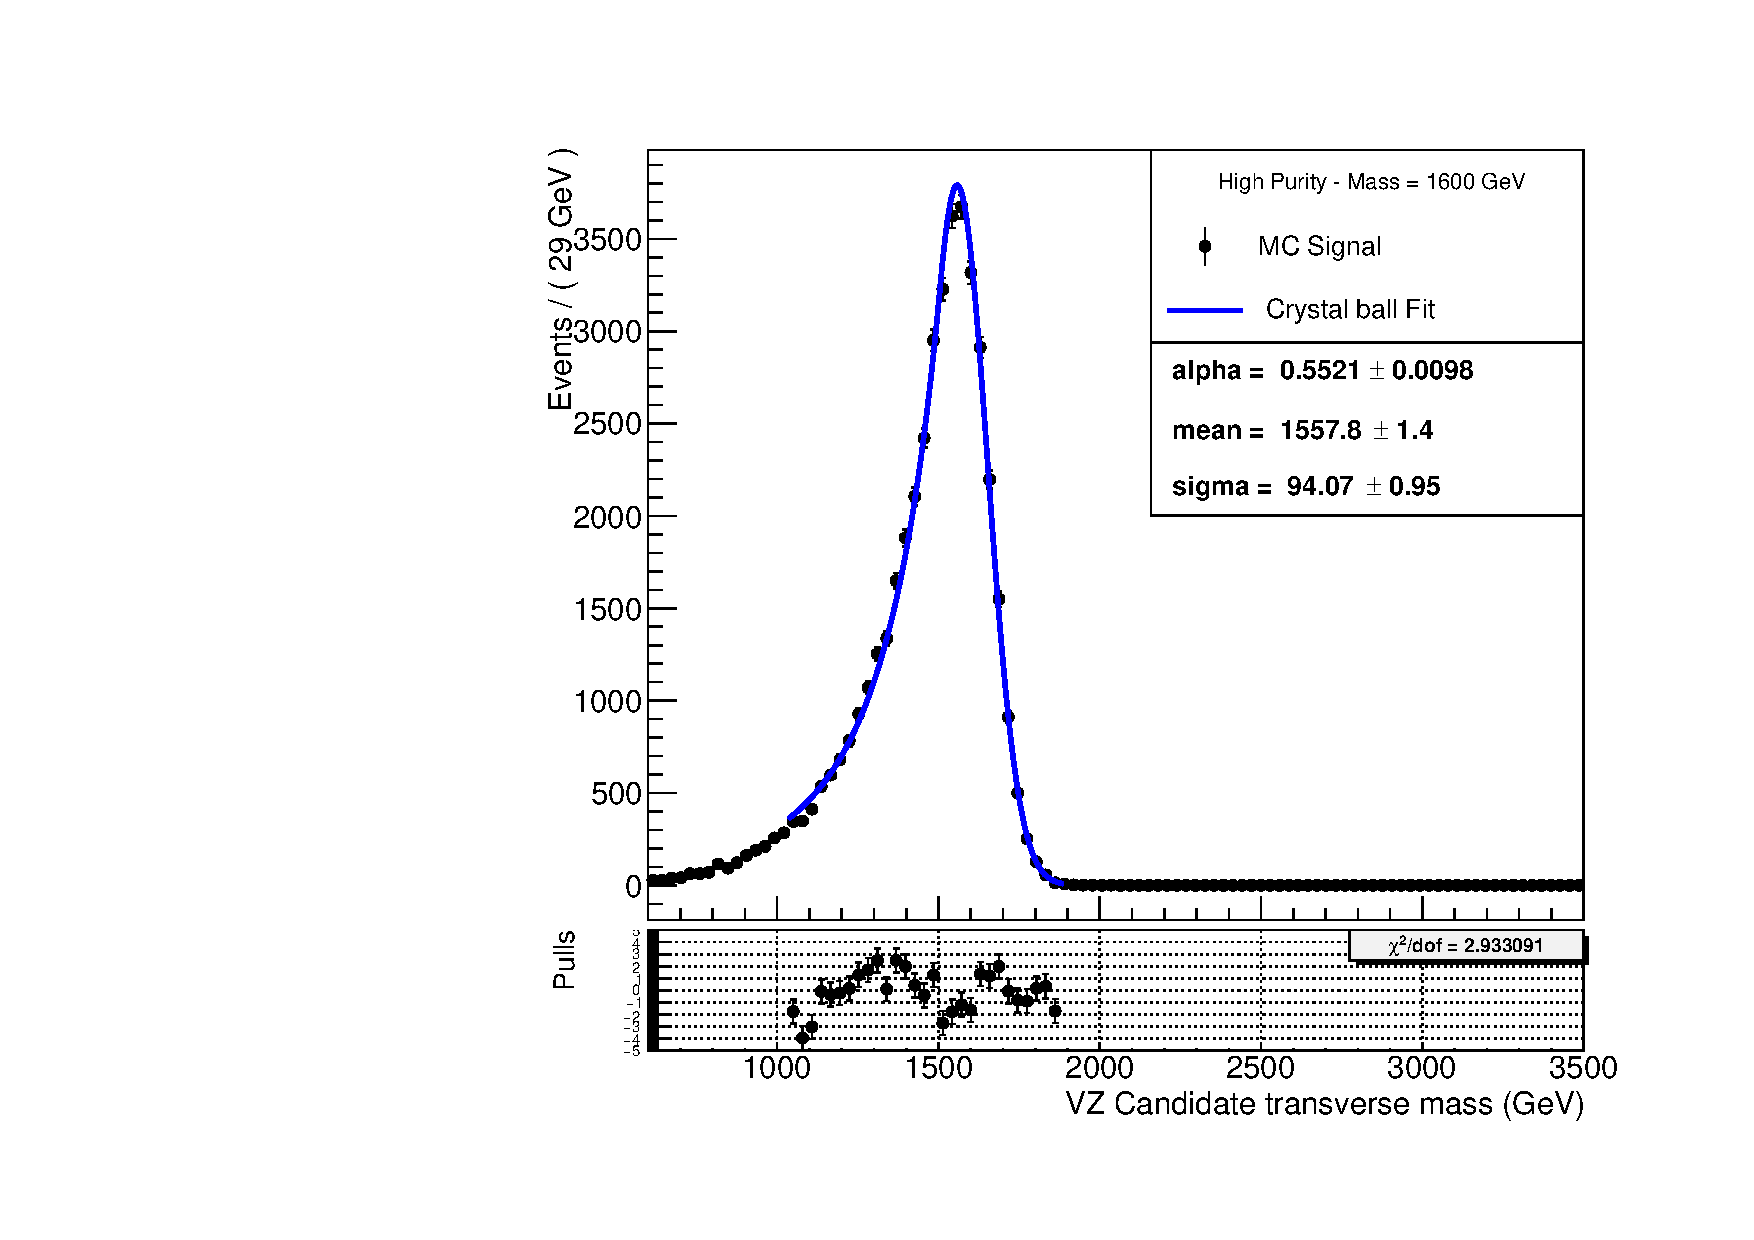
\includegraphics[width=170pt]{figuresARC/fits/BulkGravHP1600.pdf} &
  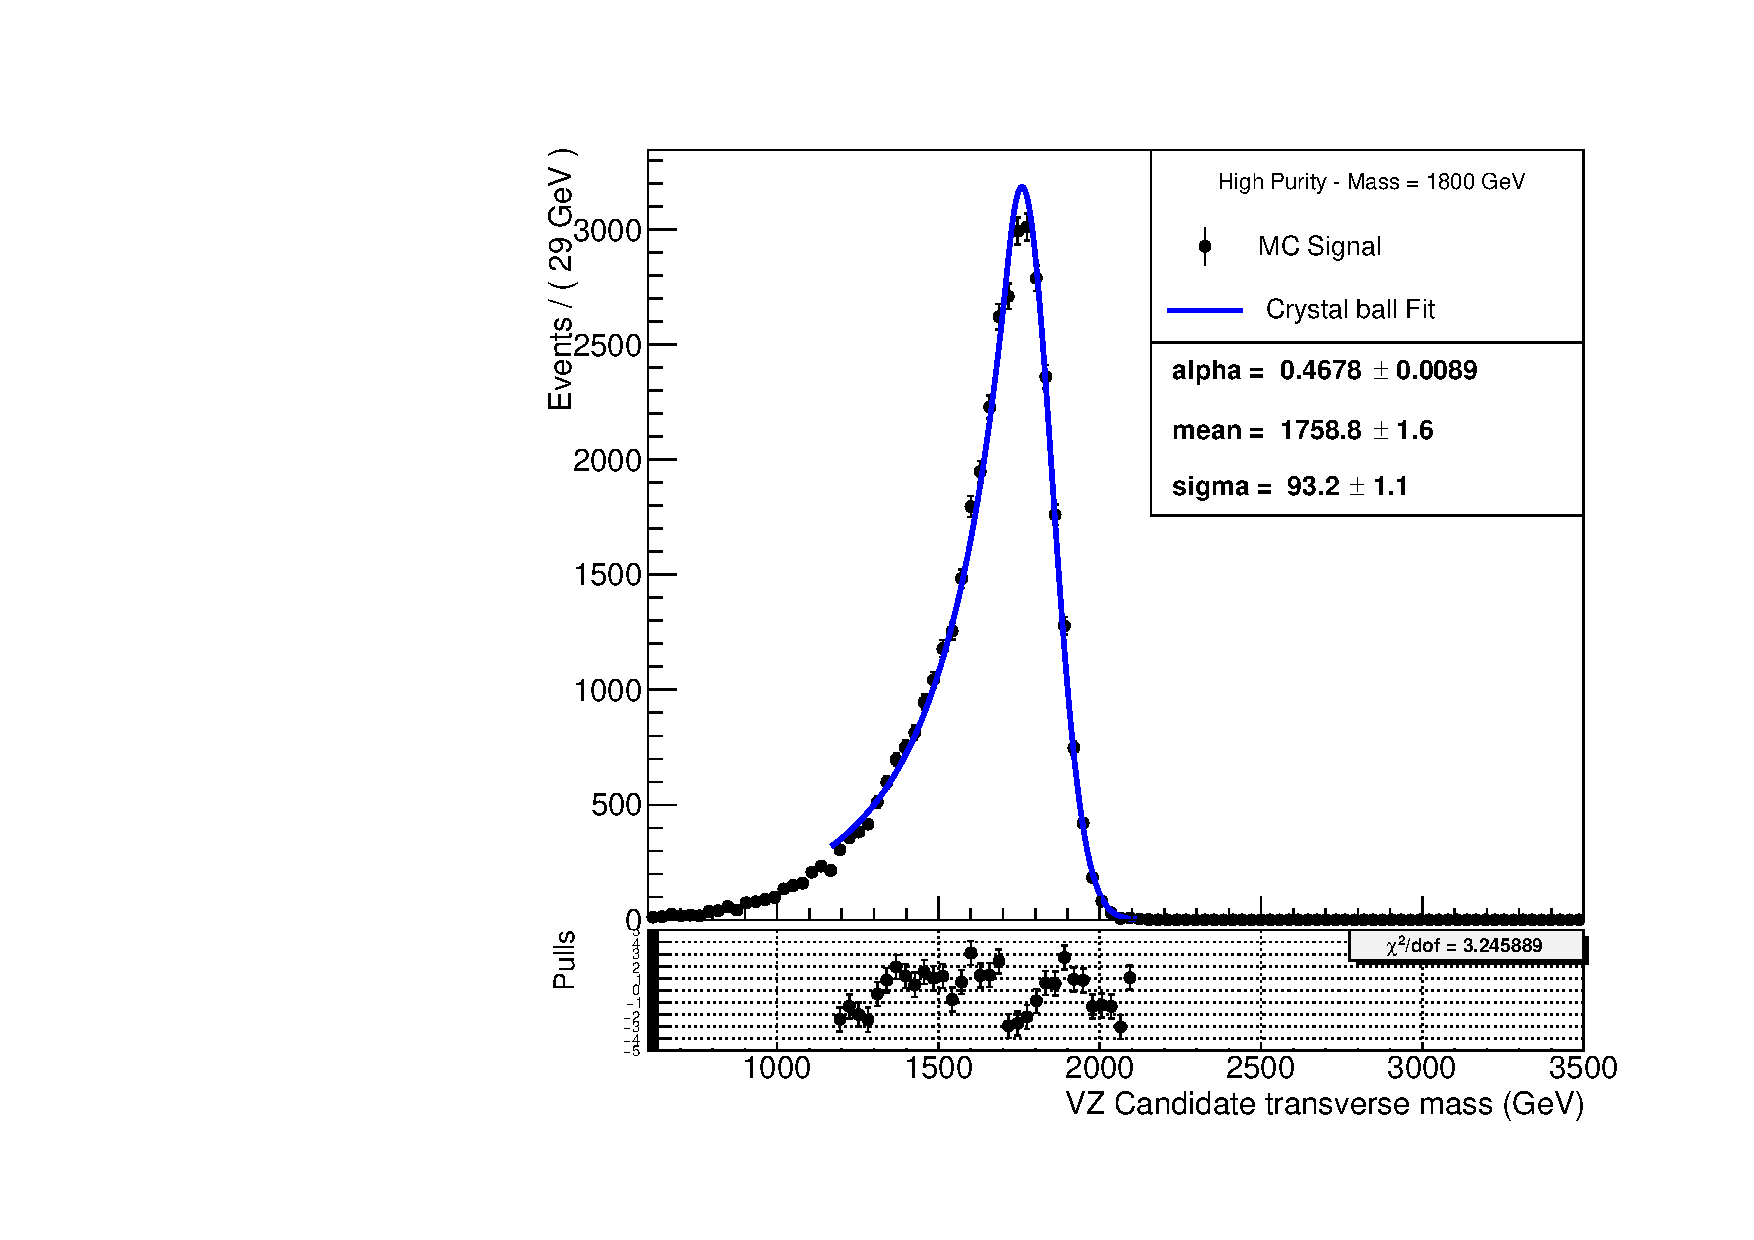
\includegraphics[width=170pt]{figuresARC/fits/BulkGravHP1800.pdf} \\
  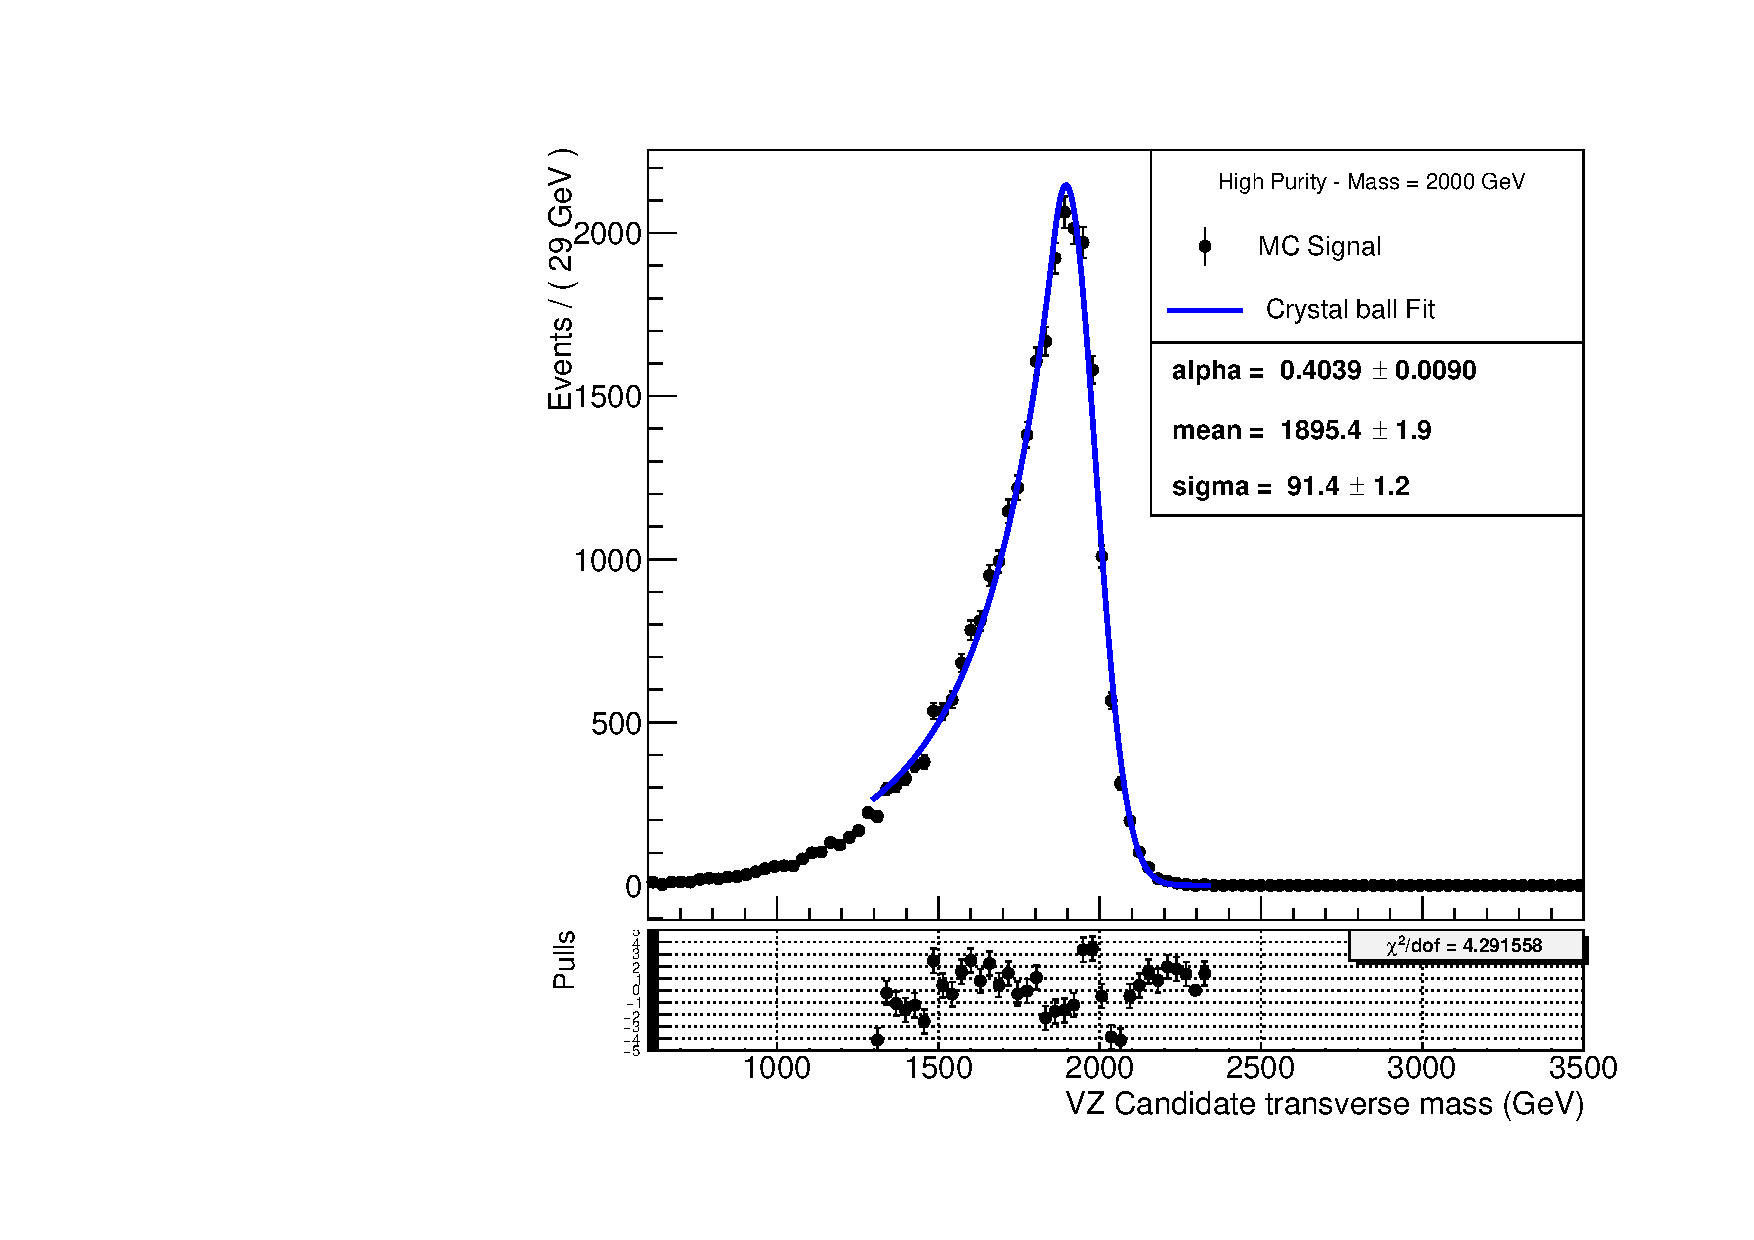
\includegraphics[width=170pt]{figuresARC/fits/BulkGravHP2000.pdf} \\ 
\end{tabular}
\label{fig:fits6a}
\end{figure}

\begin{figure}[!ht]
\caption{ Fit of the Bulk Graviton signal samples for different mass points in the LP category.}
\begin{tabular}{cc}
  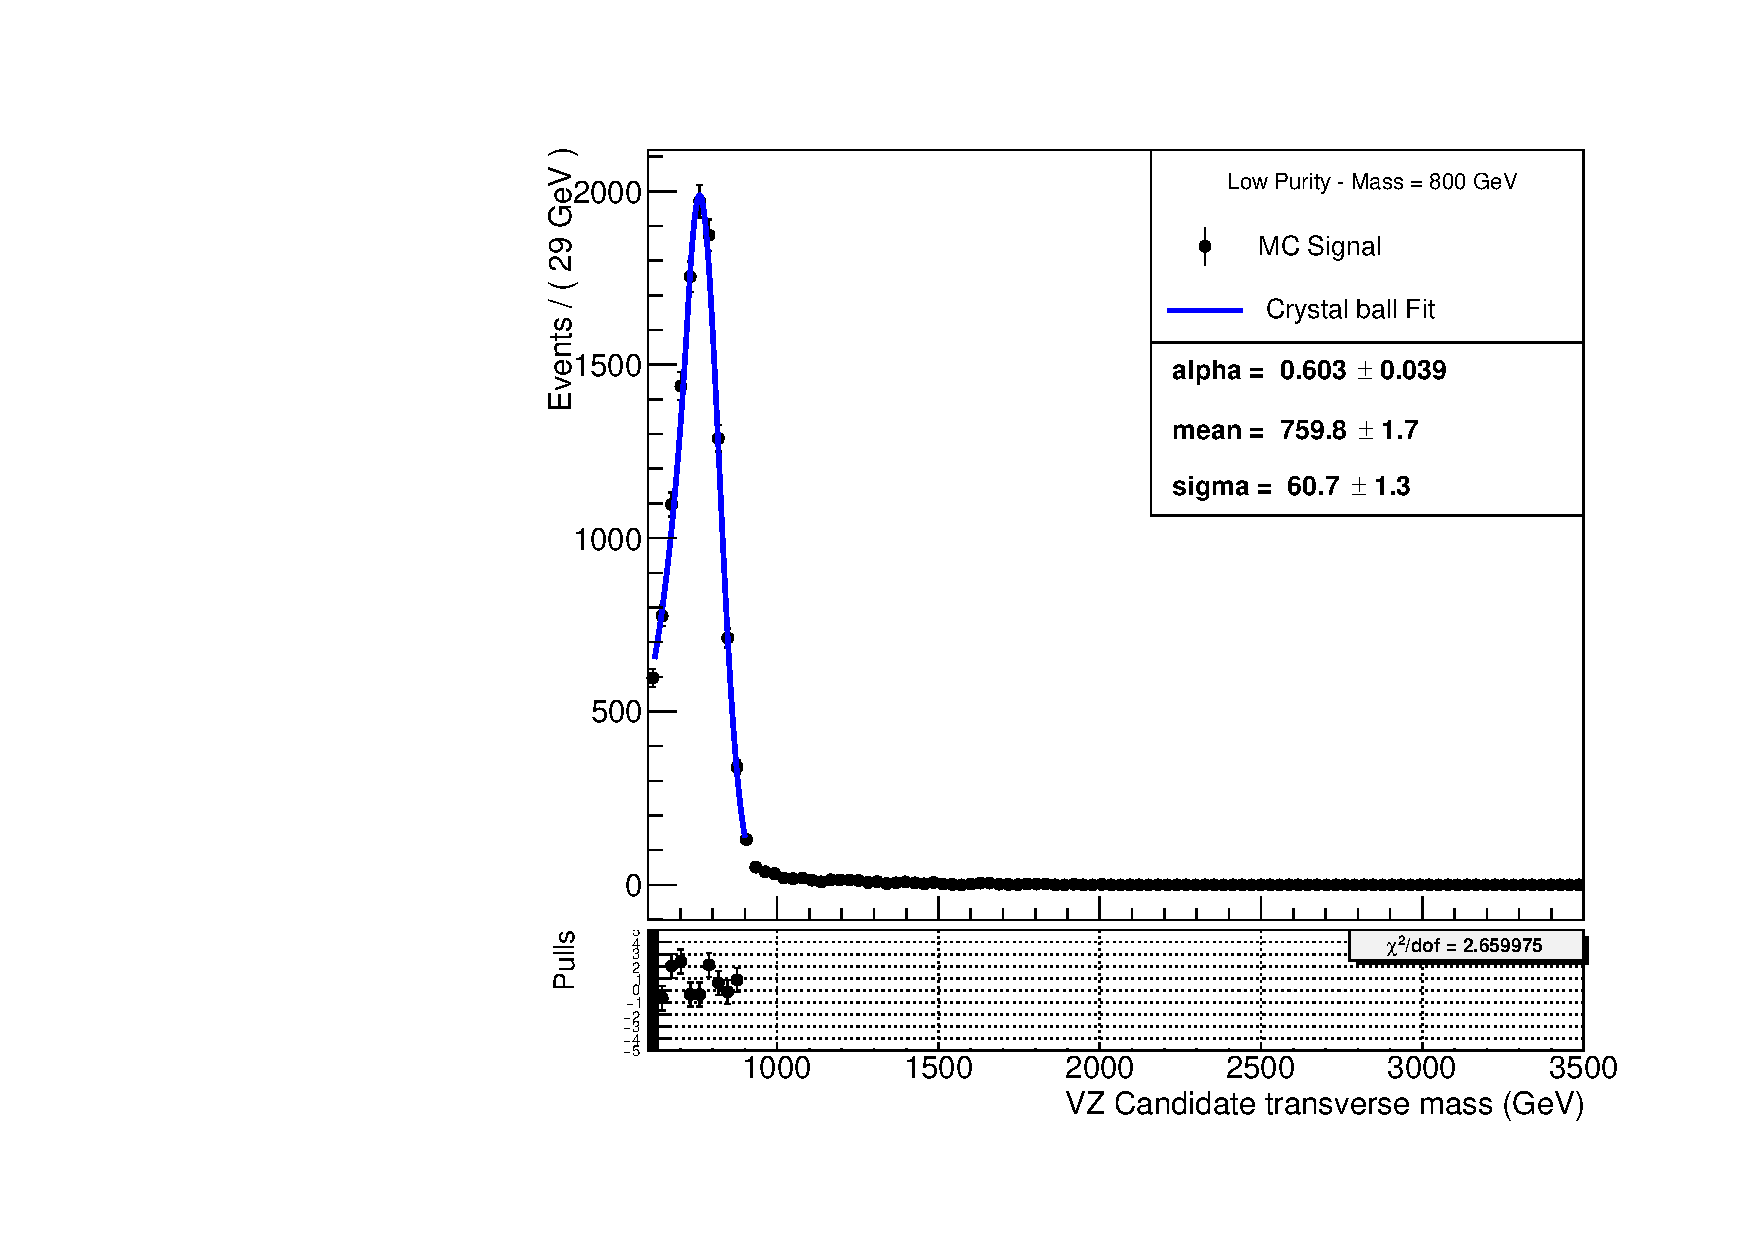
\includegraphics[width=170pt]{figuresARC/fits/BulkGravLP800.pdf} &
  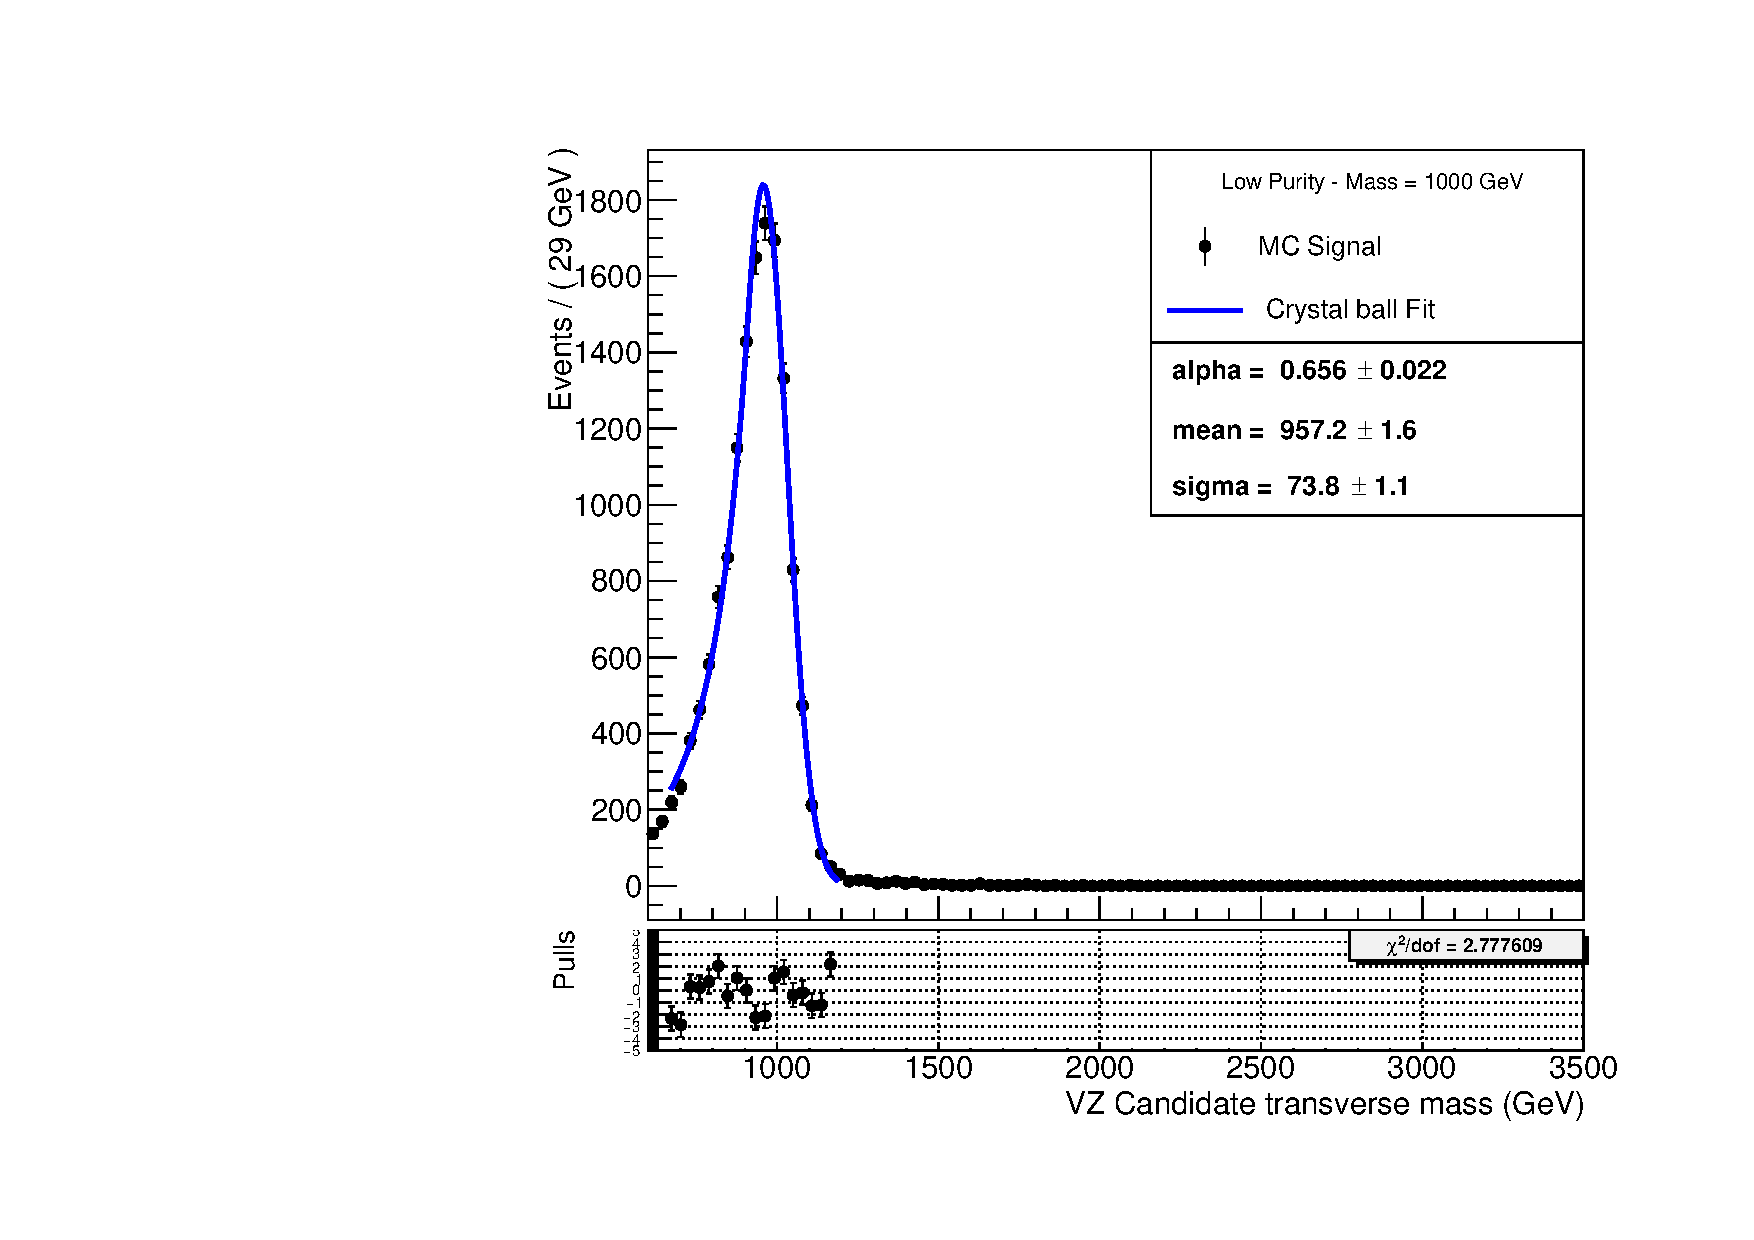
\includegraphics[width=170pt]{figuresARC/fits/BulkGravLP1000.pdf}\\
  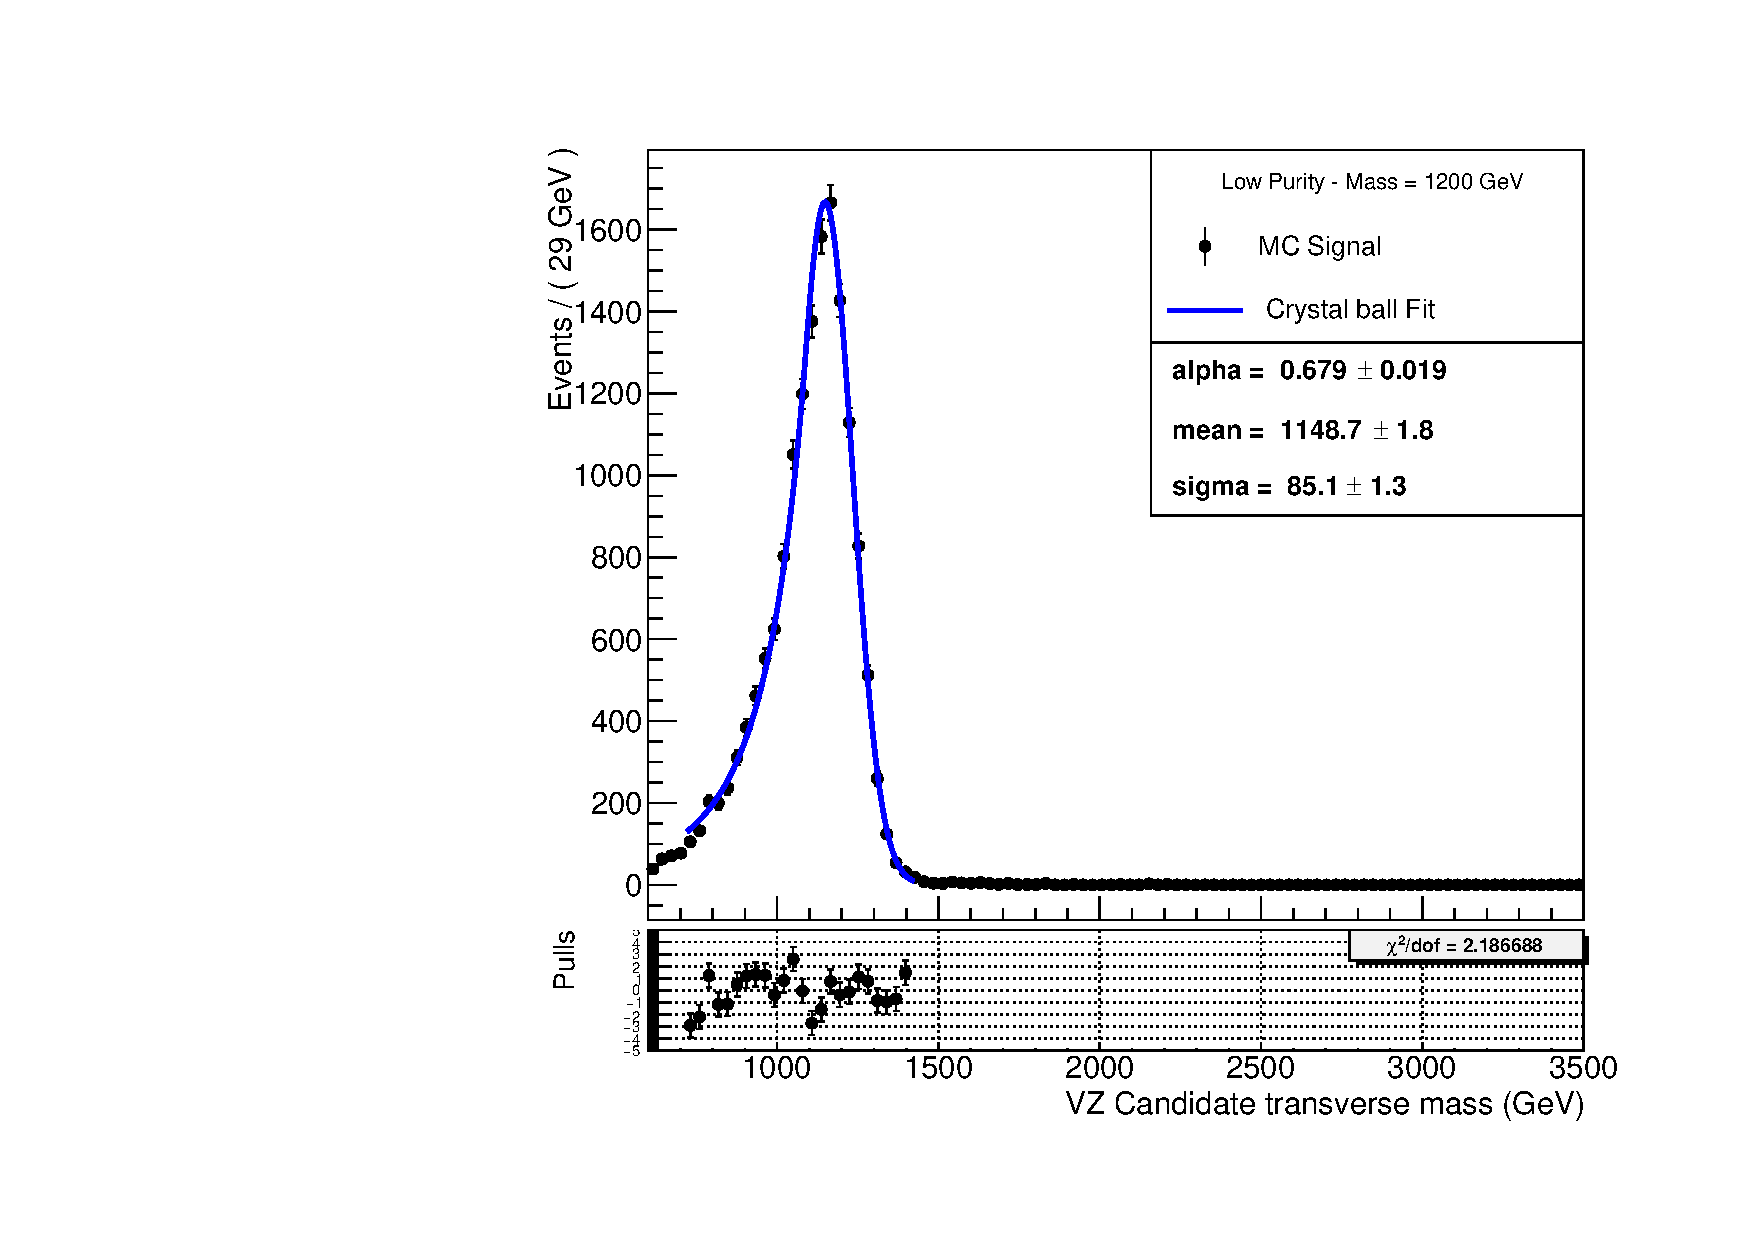
\includegraphics[width=170pt]{figuresARC/fits/BulkGravLP1200.pdf}&
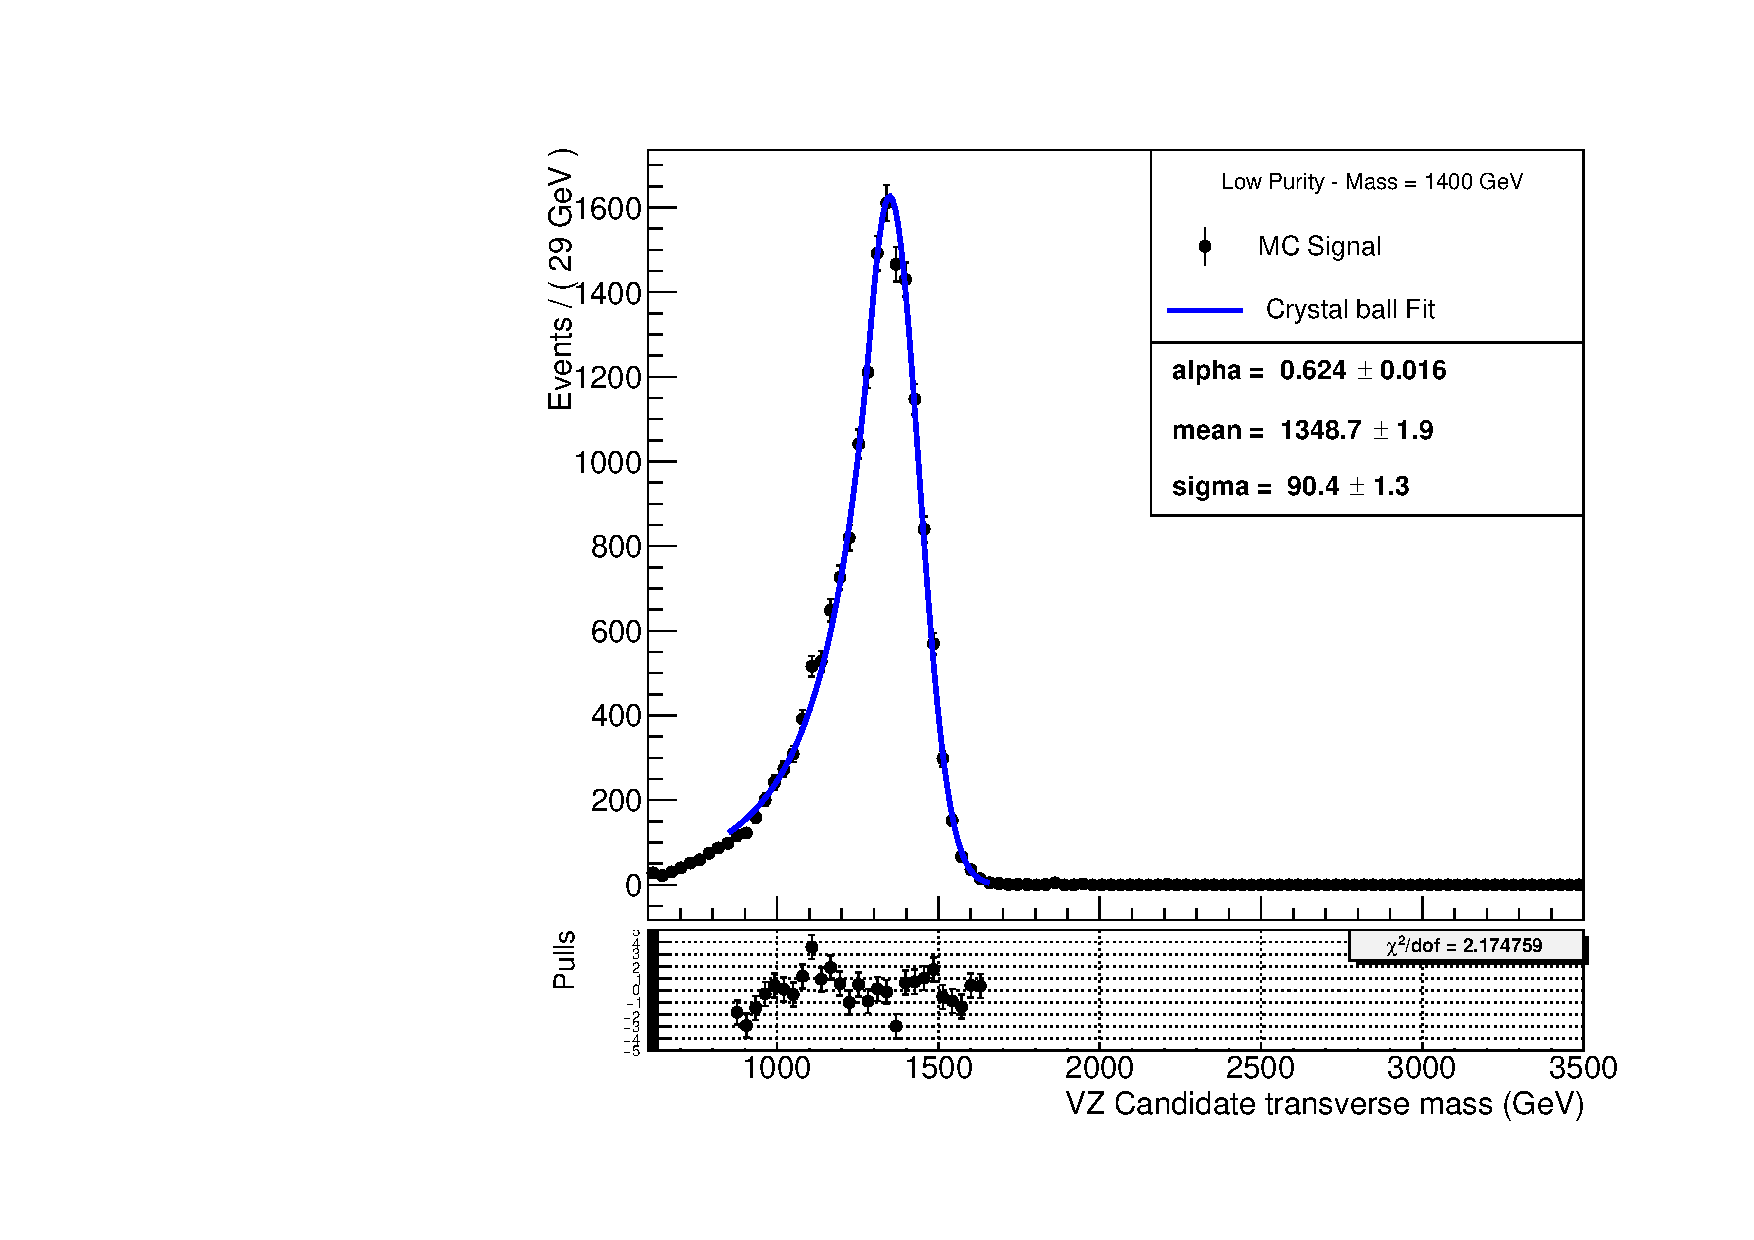
\includegraphics[width=170pt]{figuresARC/fits/BulkGravLP1400.pdf} \\
  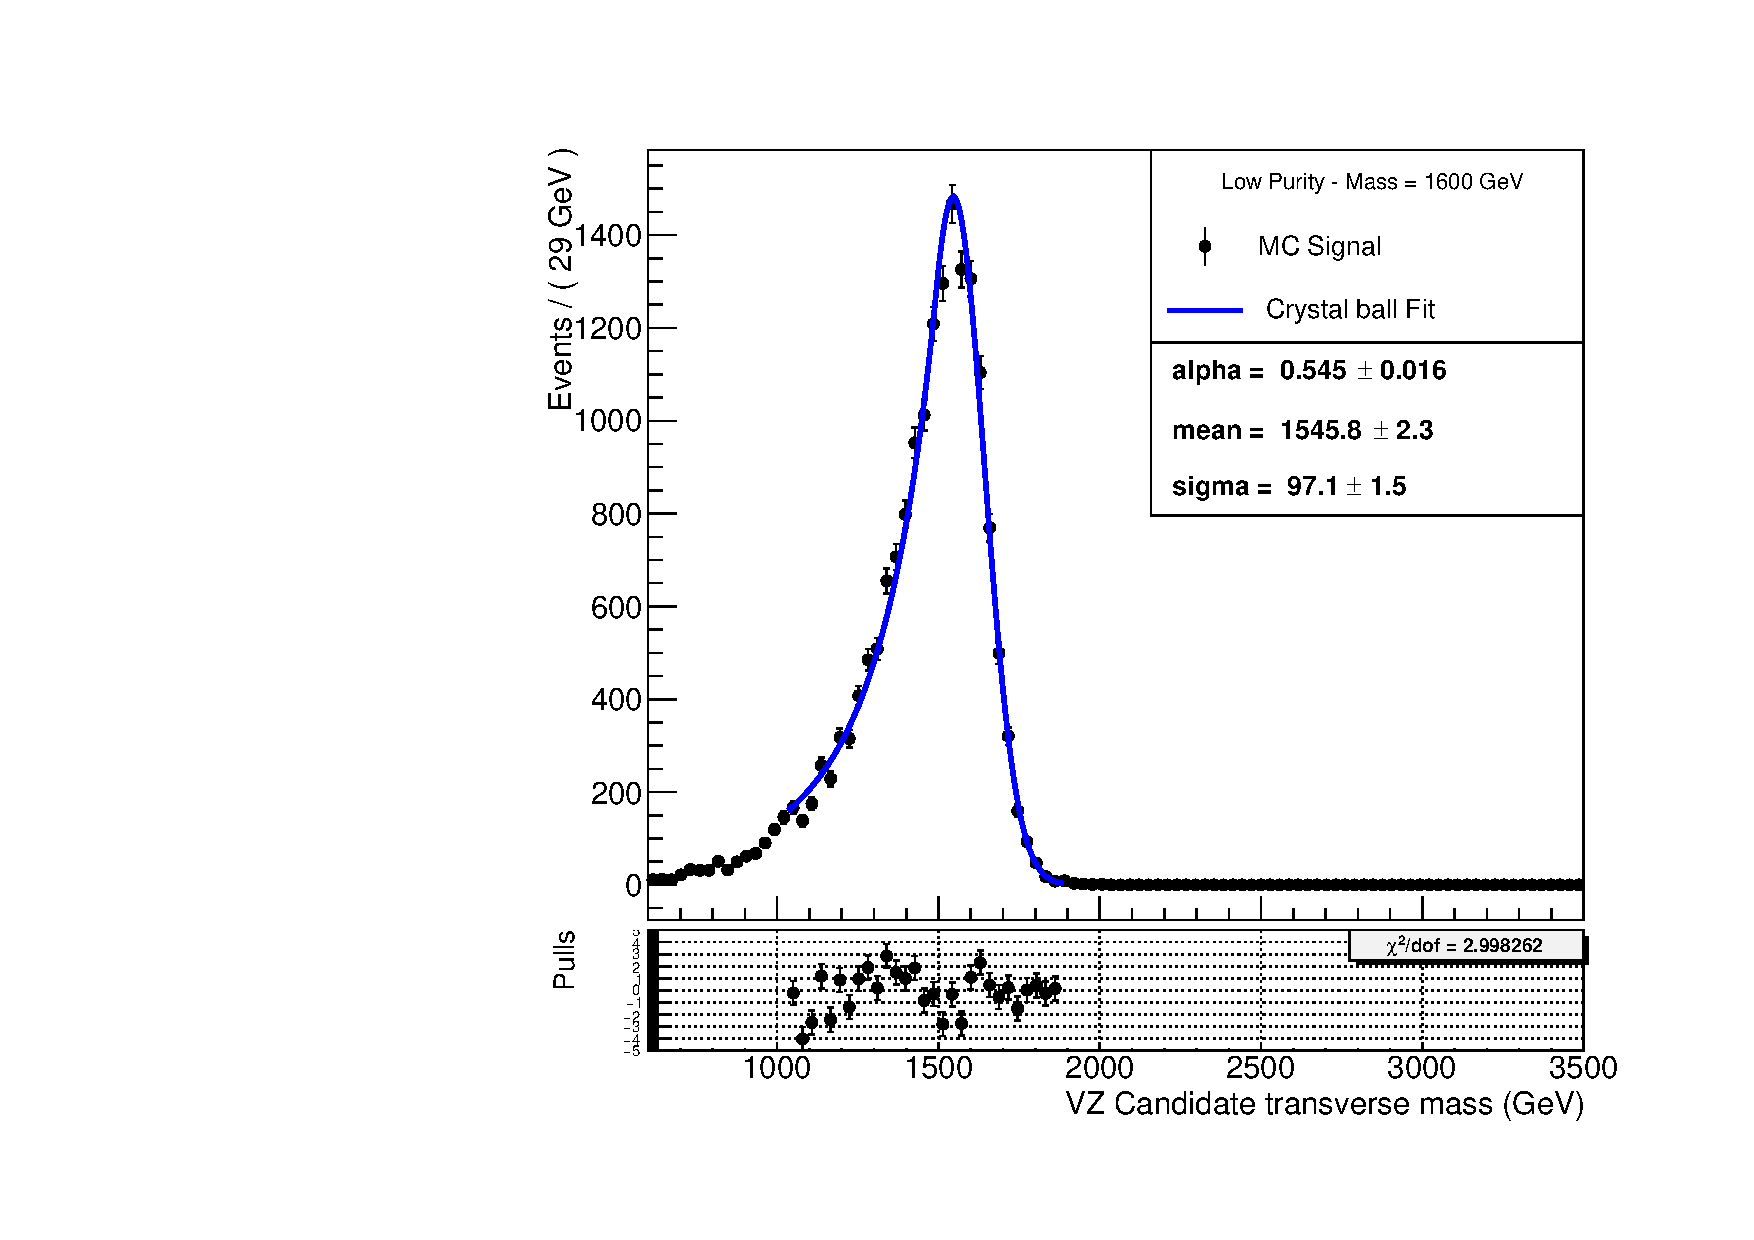
\includegraphics[width=170pt]{figuresARC/fits/BulkGravLP1600.pdf} &
  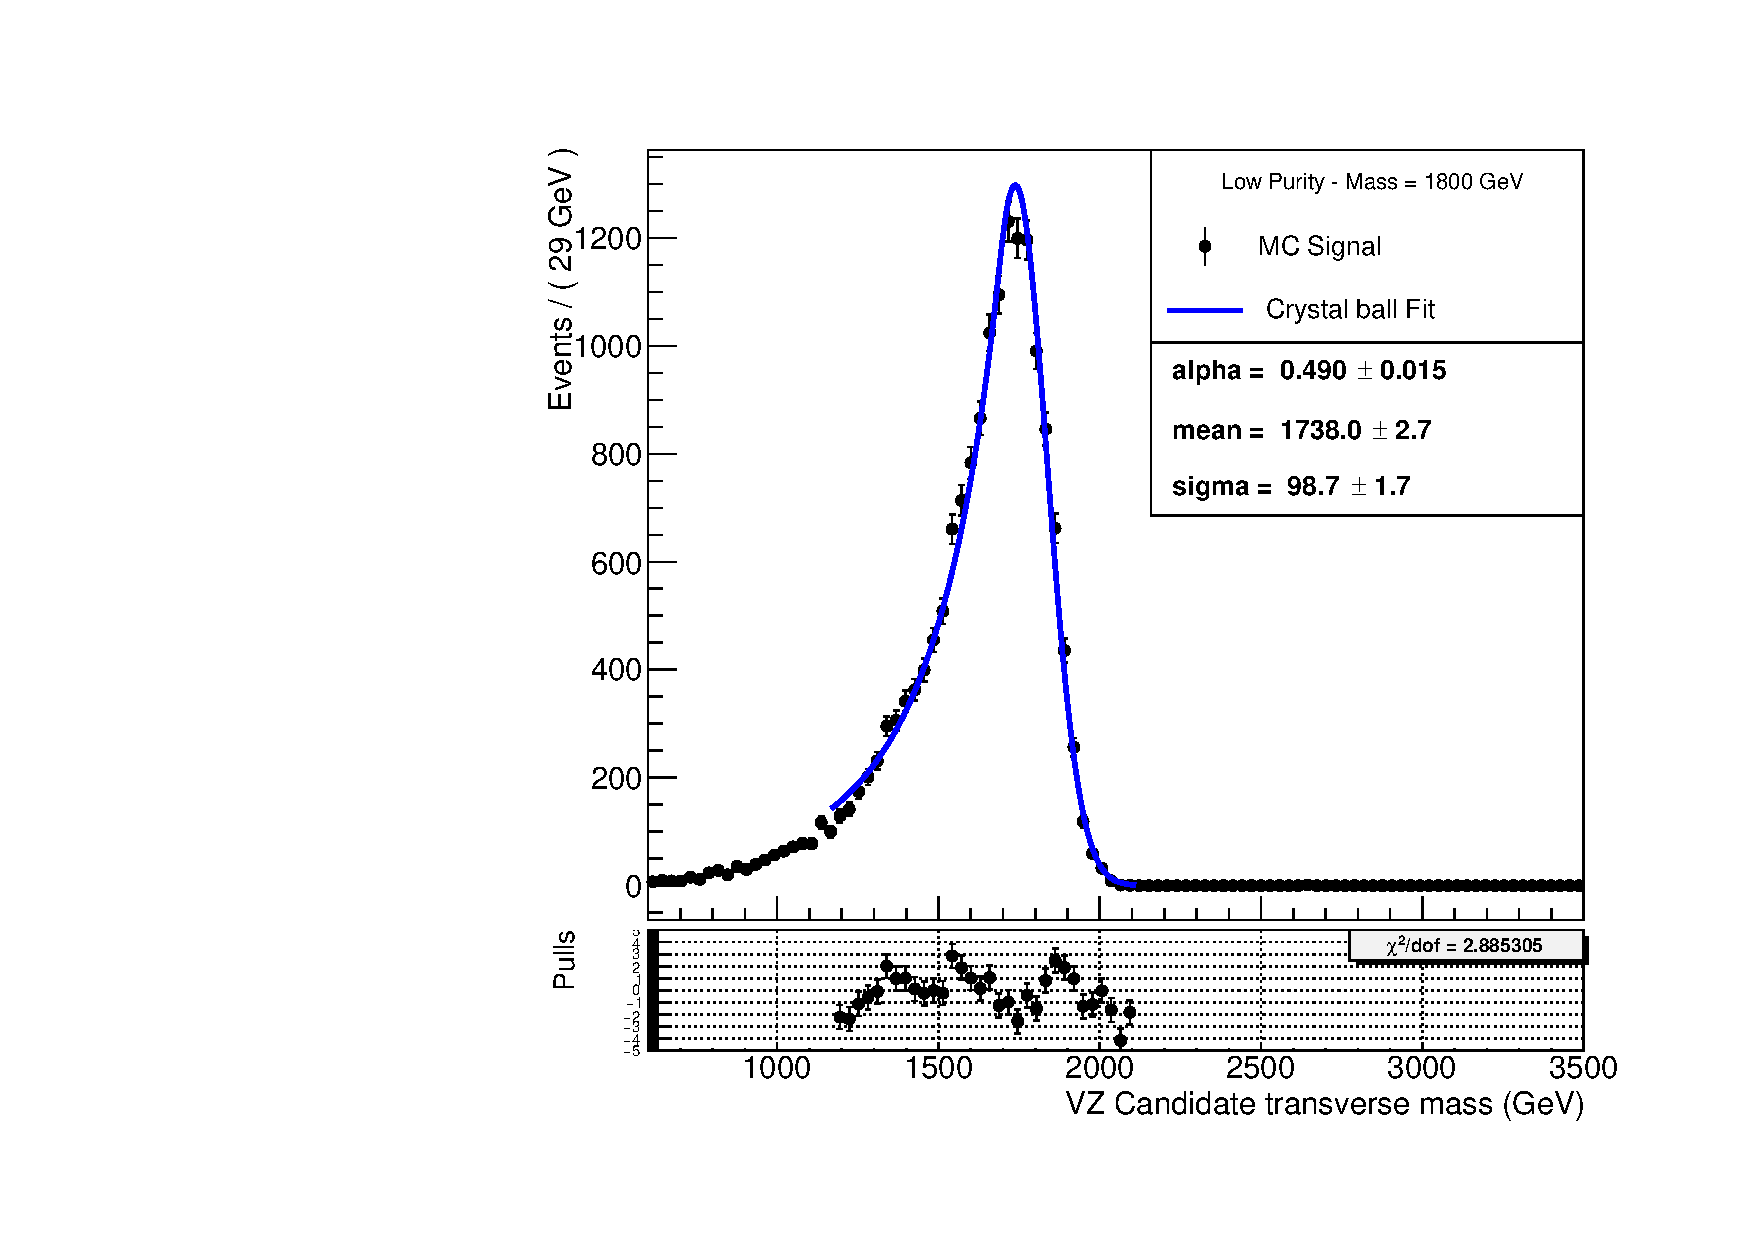
\includegraphics[width=170pt]{figuresARC/fits/BulkGravLP1800.pdf} \\
  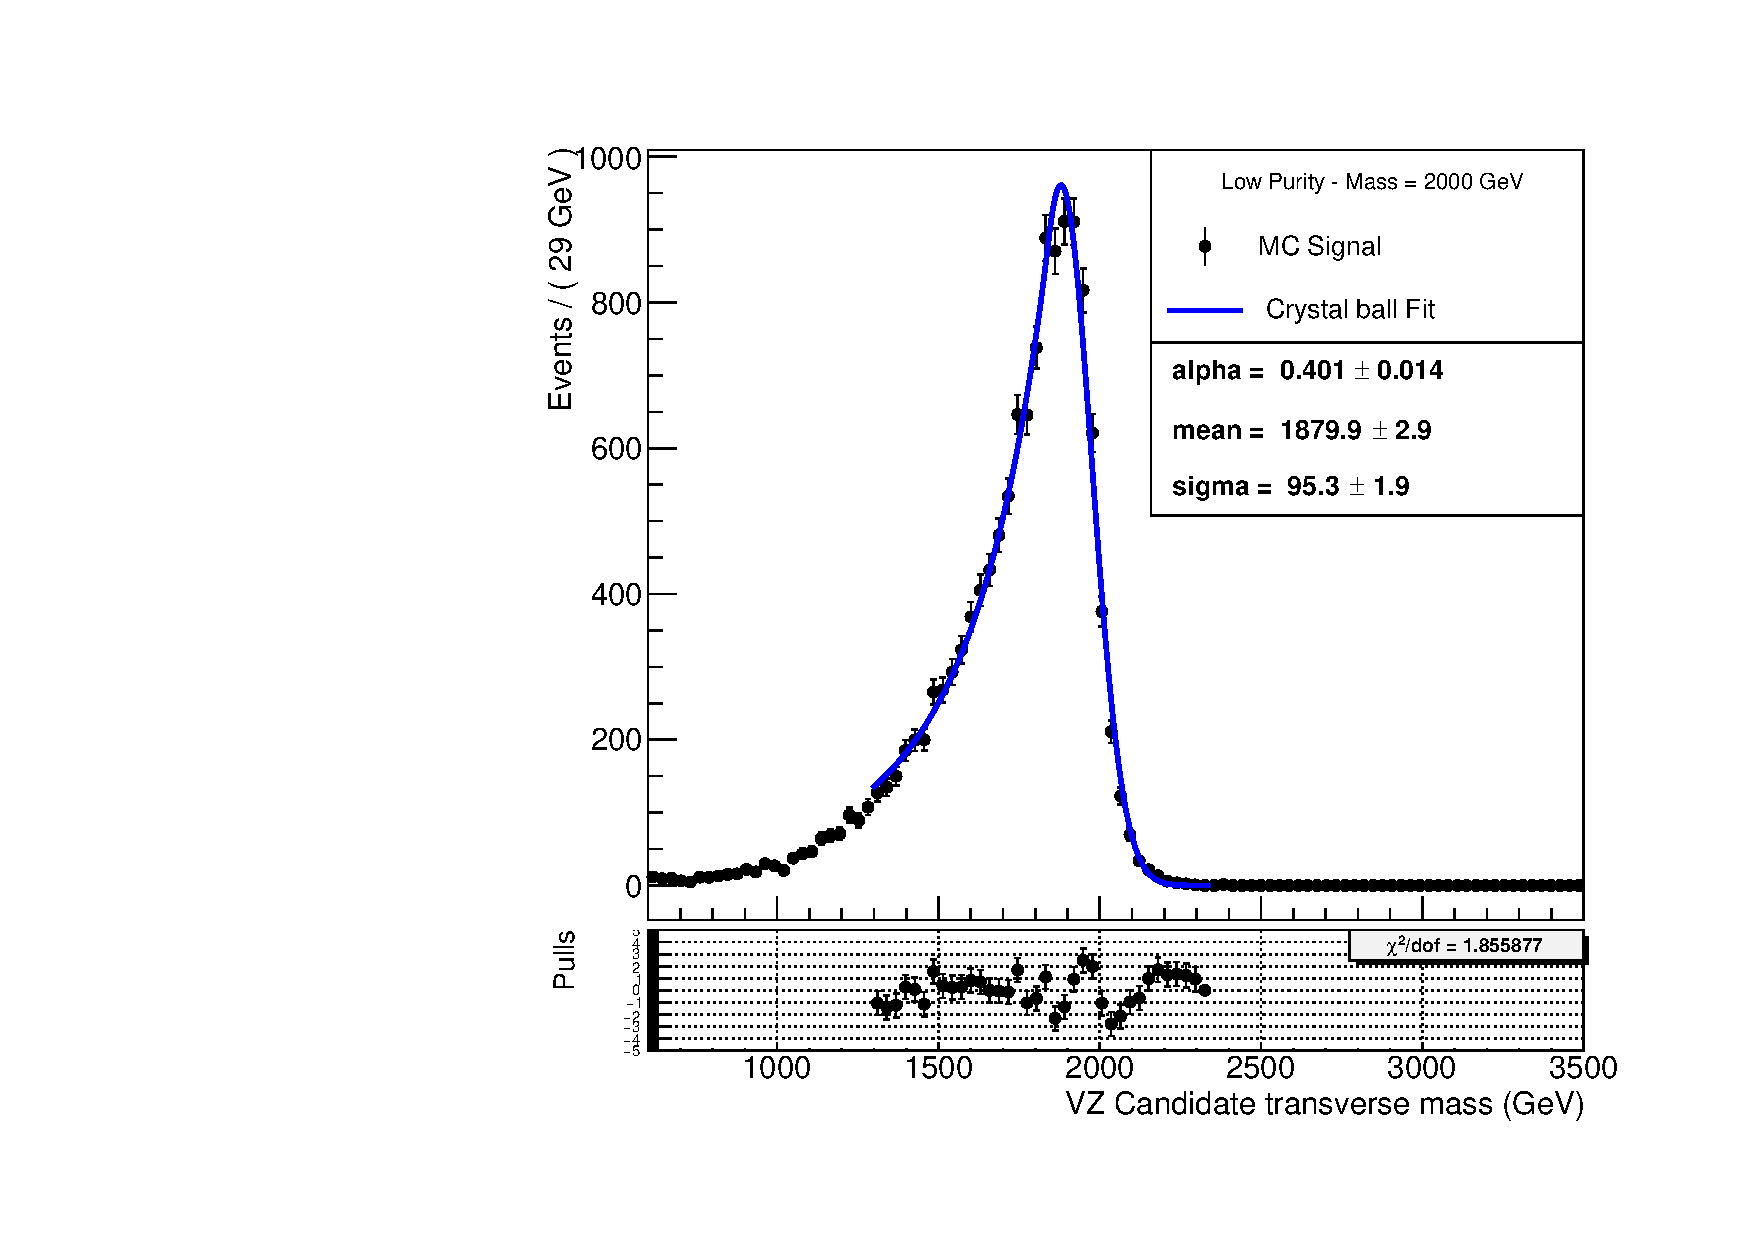
\includegraphics[width=170pt]{figuresARC/fits/BulkGravLP2000.pdf} \\
\end{tabular}
\label{fig:fits6b}
\end{figure}


\begin{figure}[!ht]
\caption{ Top: Fit of the W prime signal samples for different mass points in the HP category. Bottom: Fit of the W prime signal samples for different mass points in the LP category}
\begin{tabular}{ccc}
  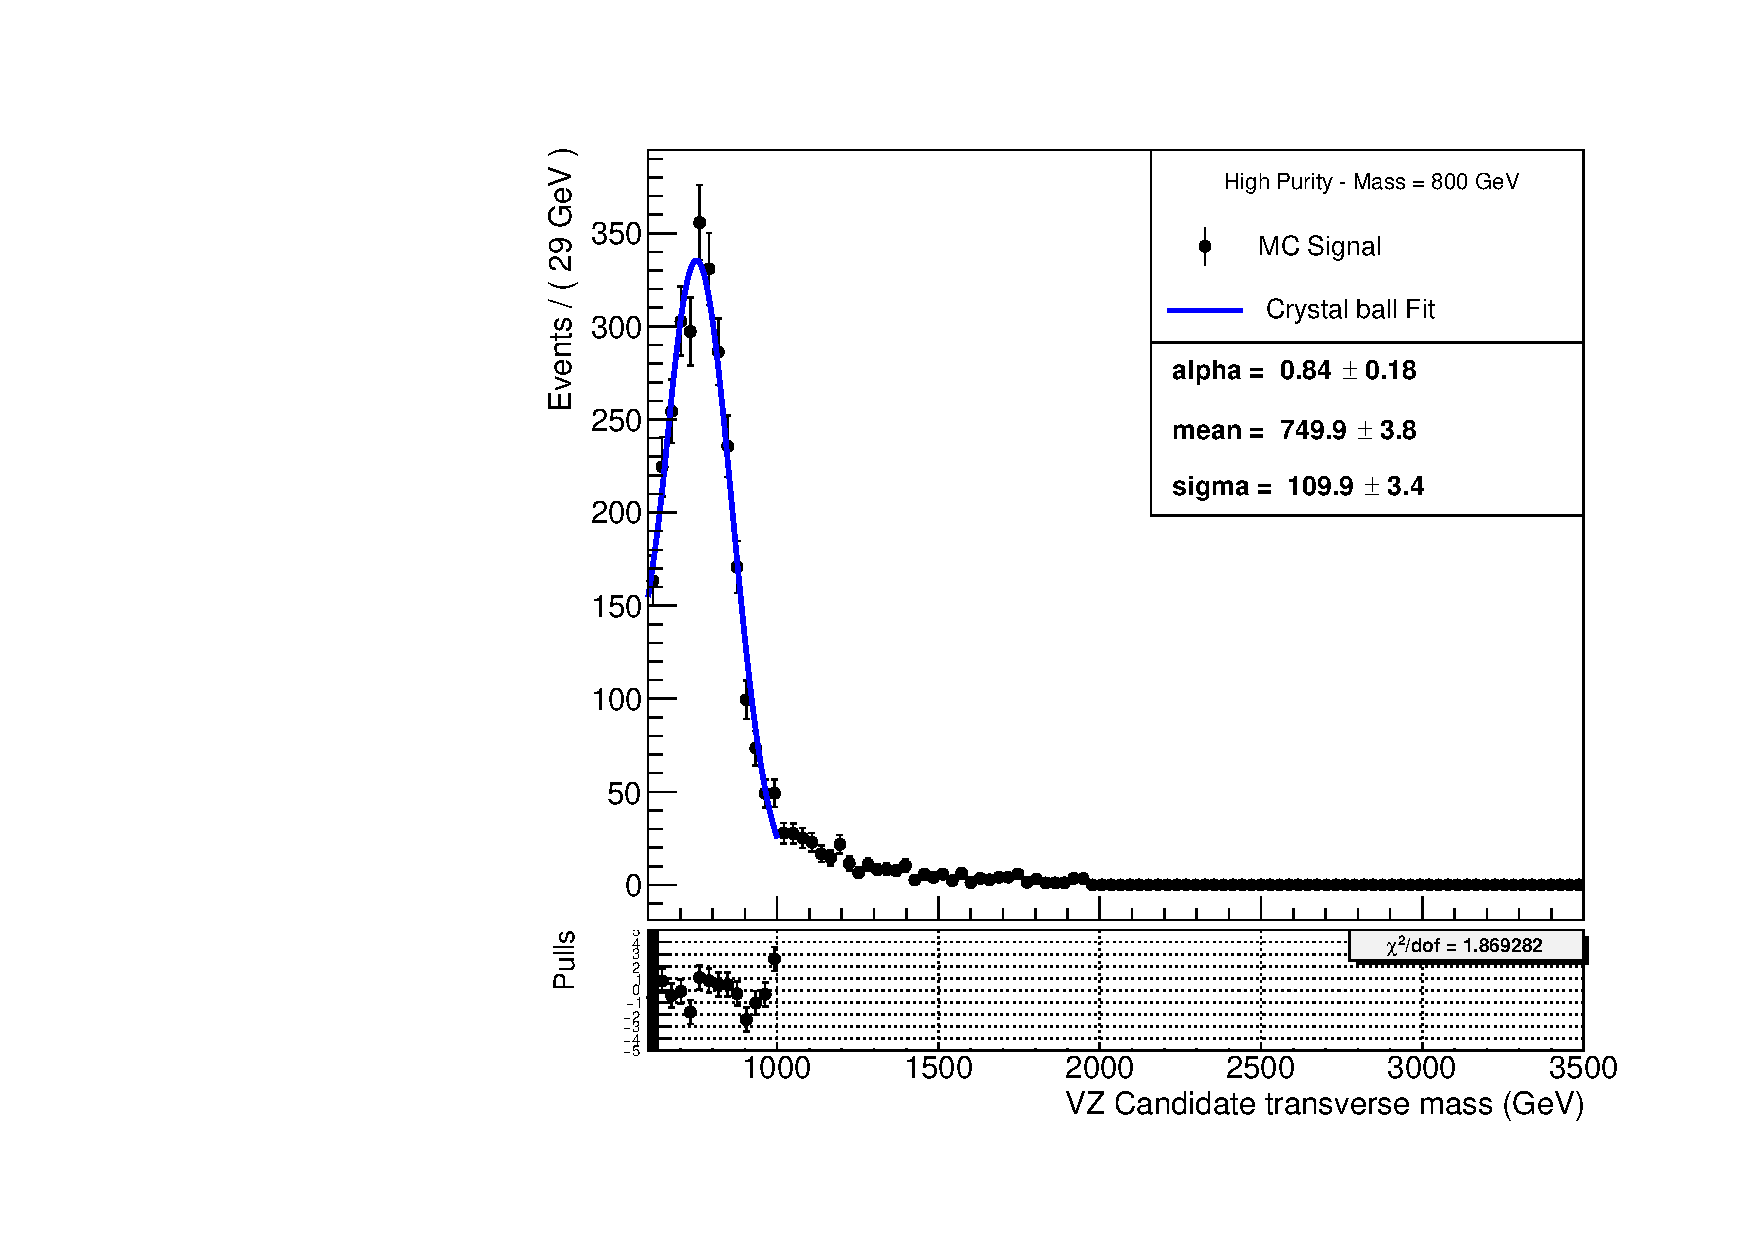
\includegraphics[width=150pt]{figuresARC/fits/WprimeHP800.pdf} &
  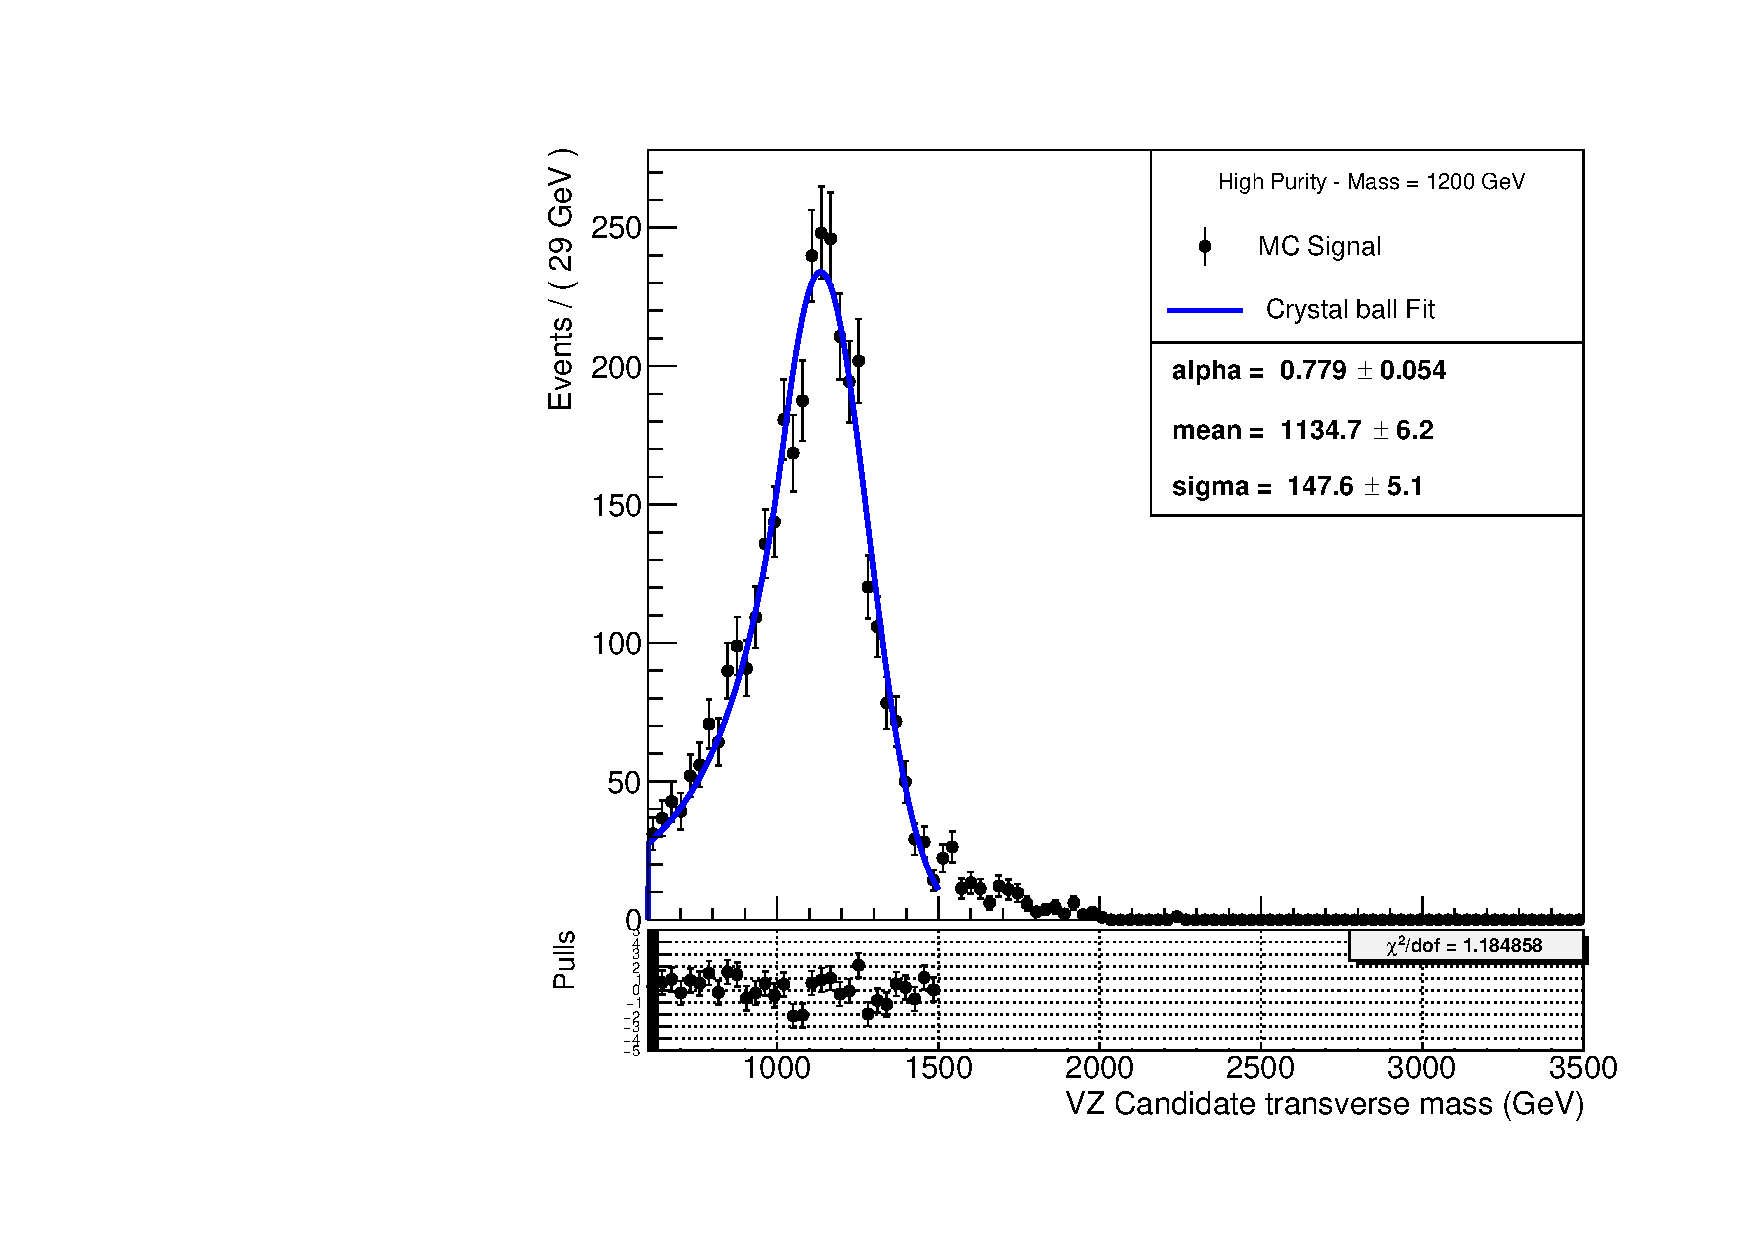
\includegraphics[width=150pt]{figuresARC/fits/WprimeHP1200.pdf} & 
  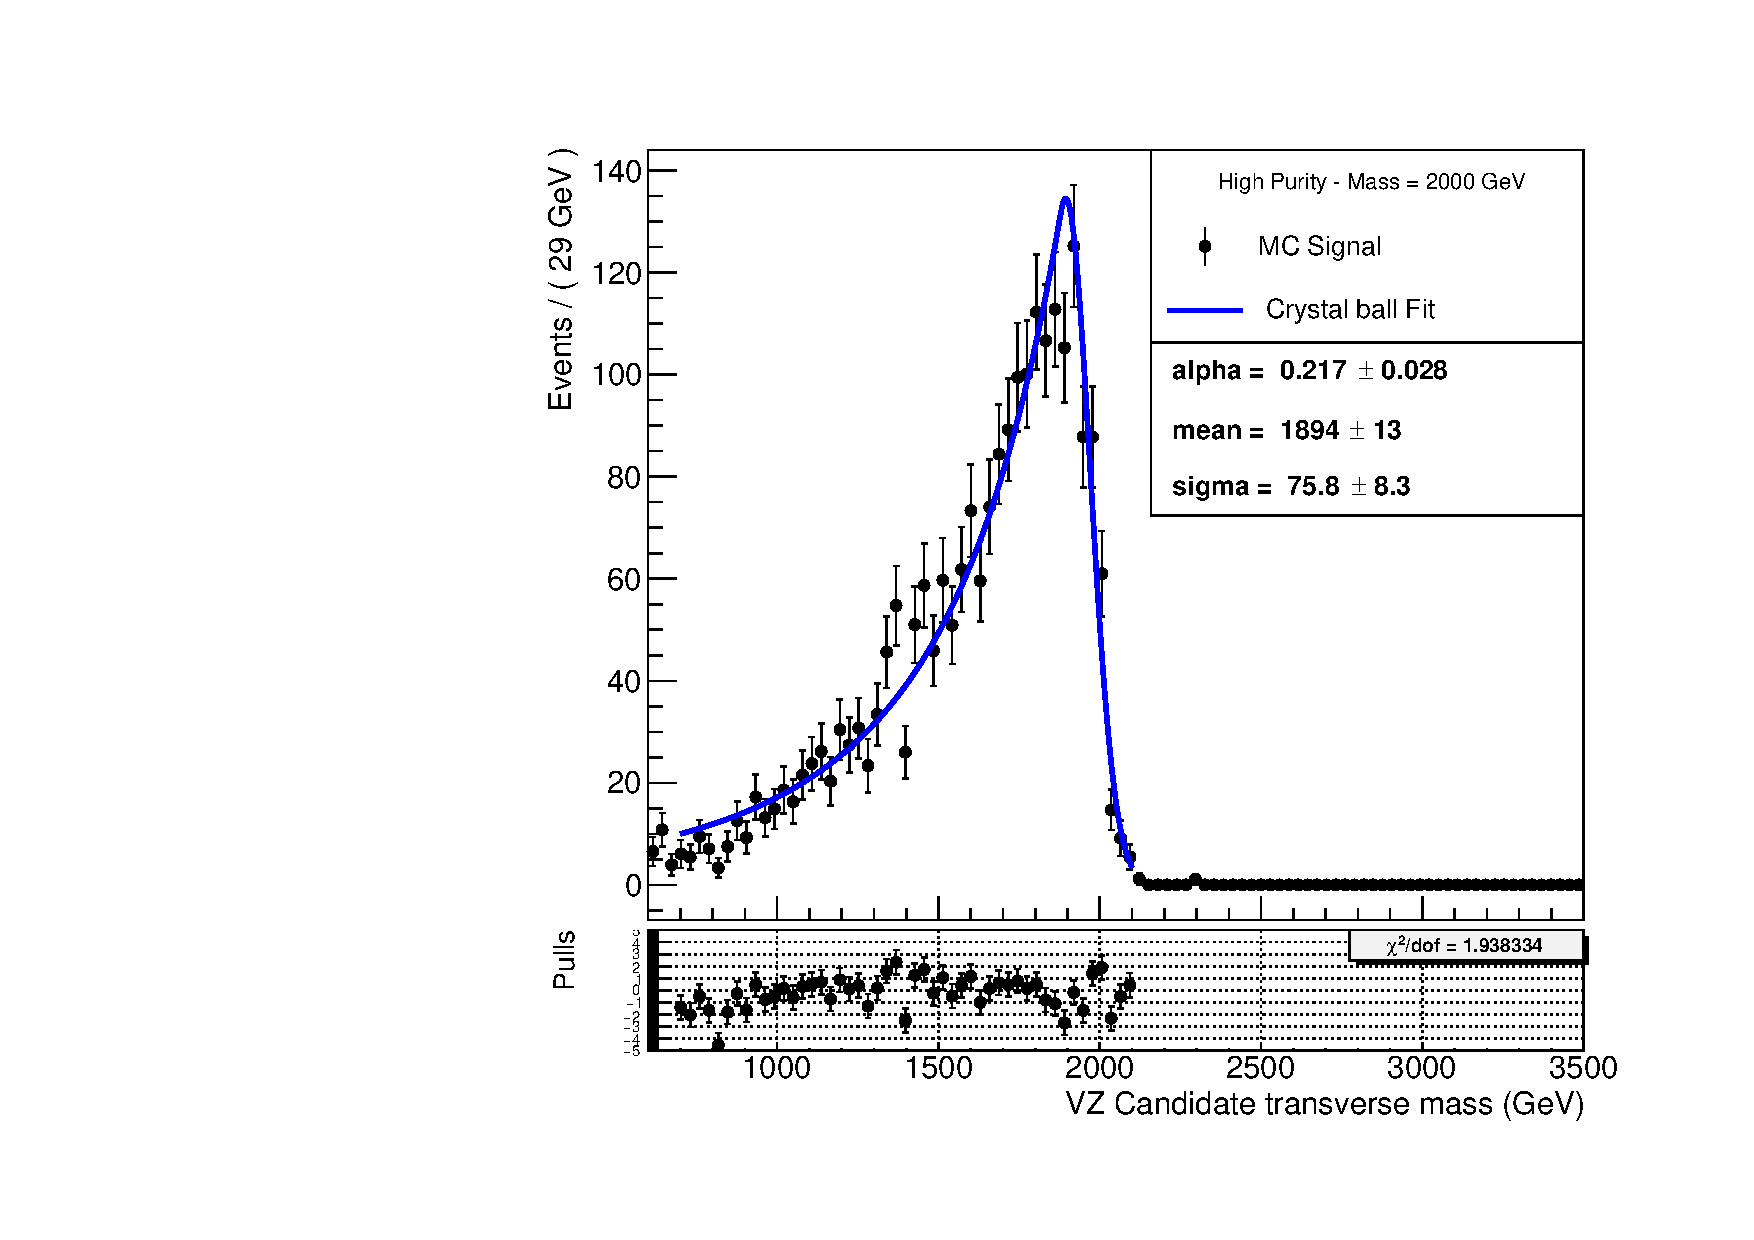
\includegraphics[width=150pt]{figuresARC/fits/WprimeHP2000.pdf}\\
    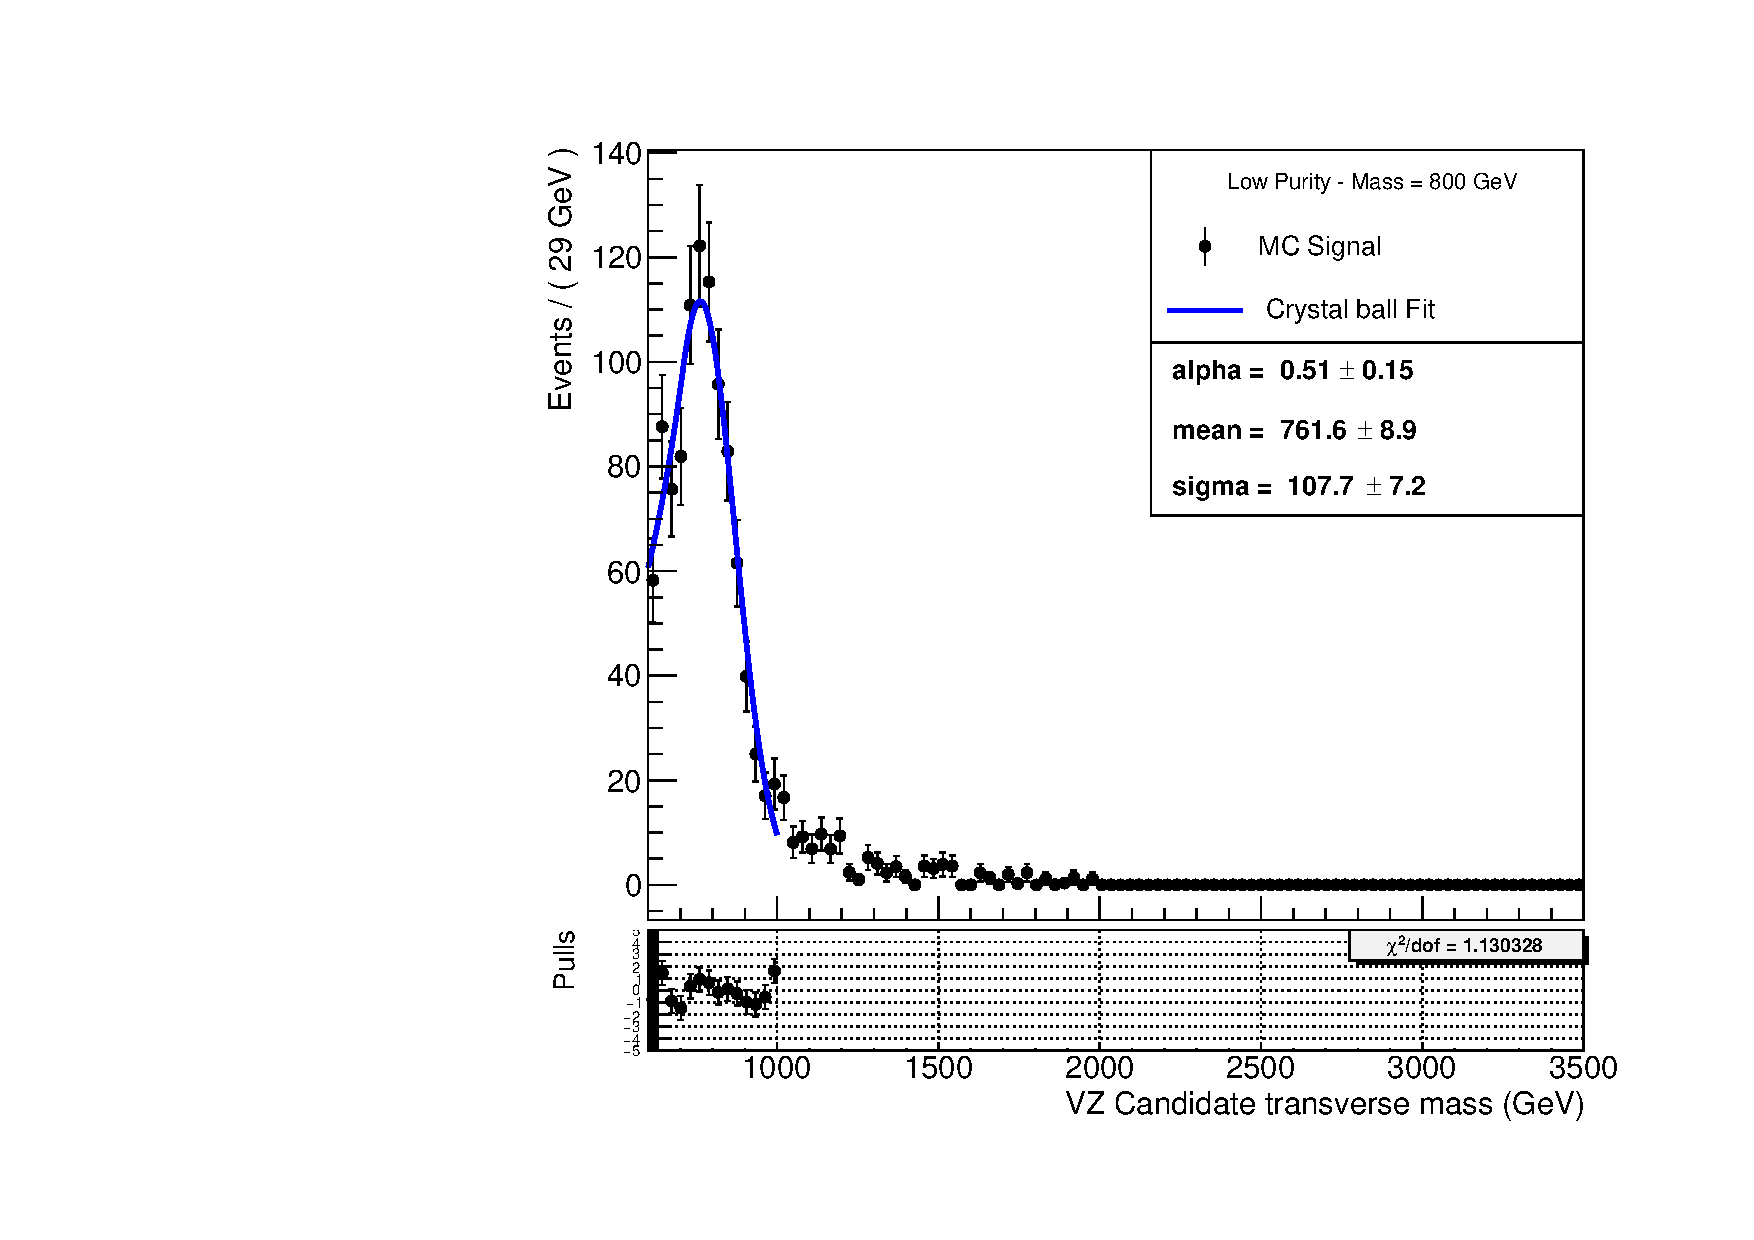
\includegraphics[width=150pt]{figuresARC/fits/WprimeLP800.pdf} &
    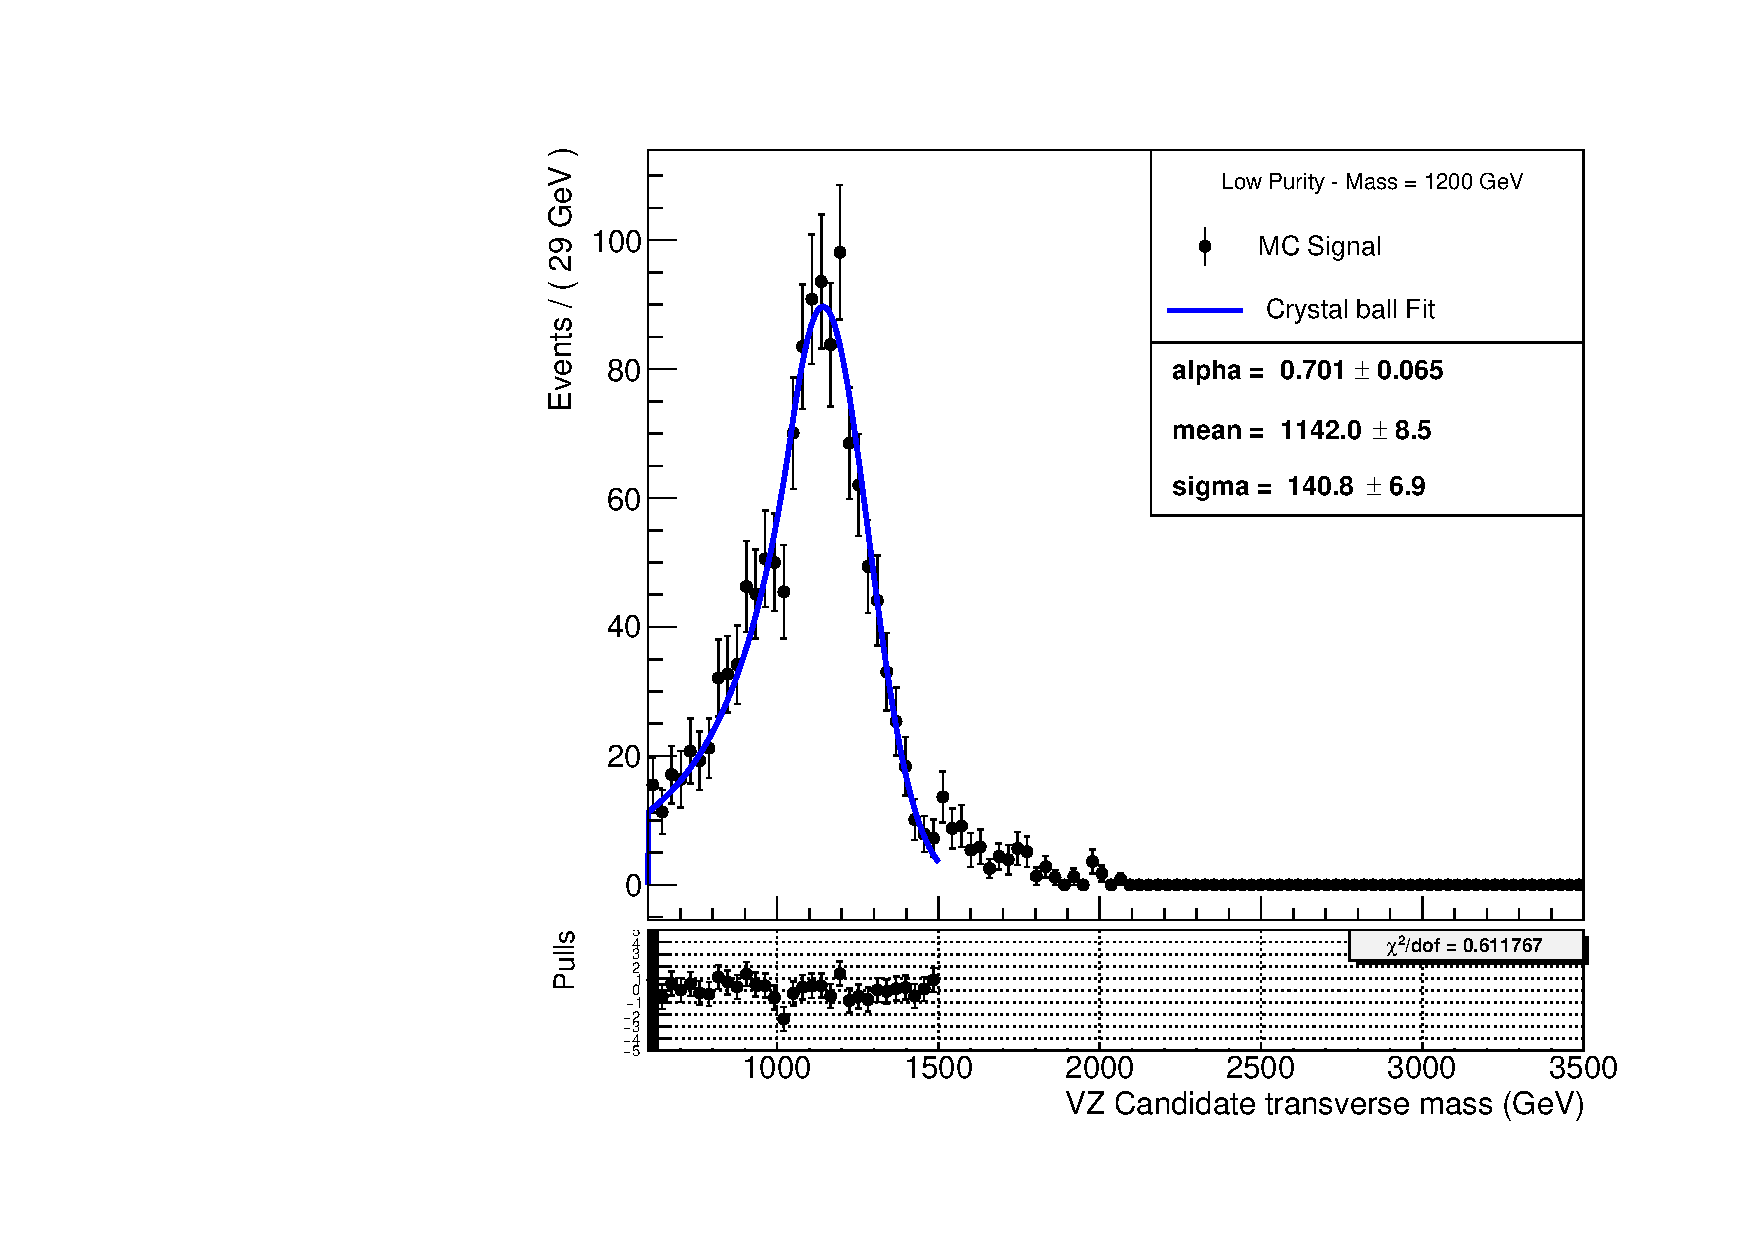
\includegraphics[width=150pt]{figuresARC/fits/WprimeLP1200.pdf} &
    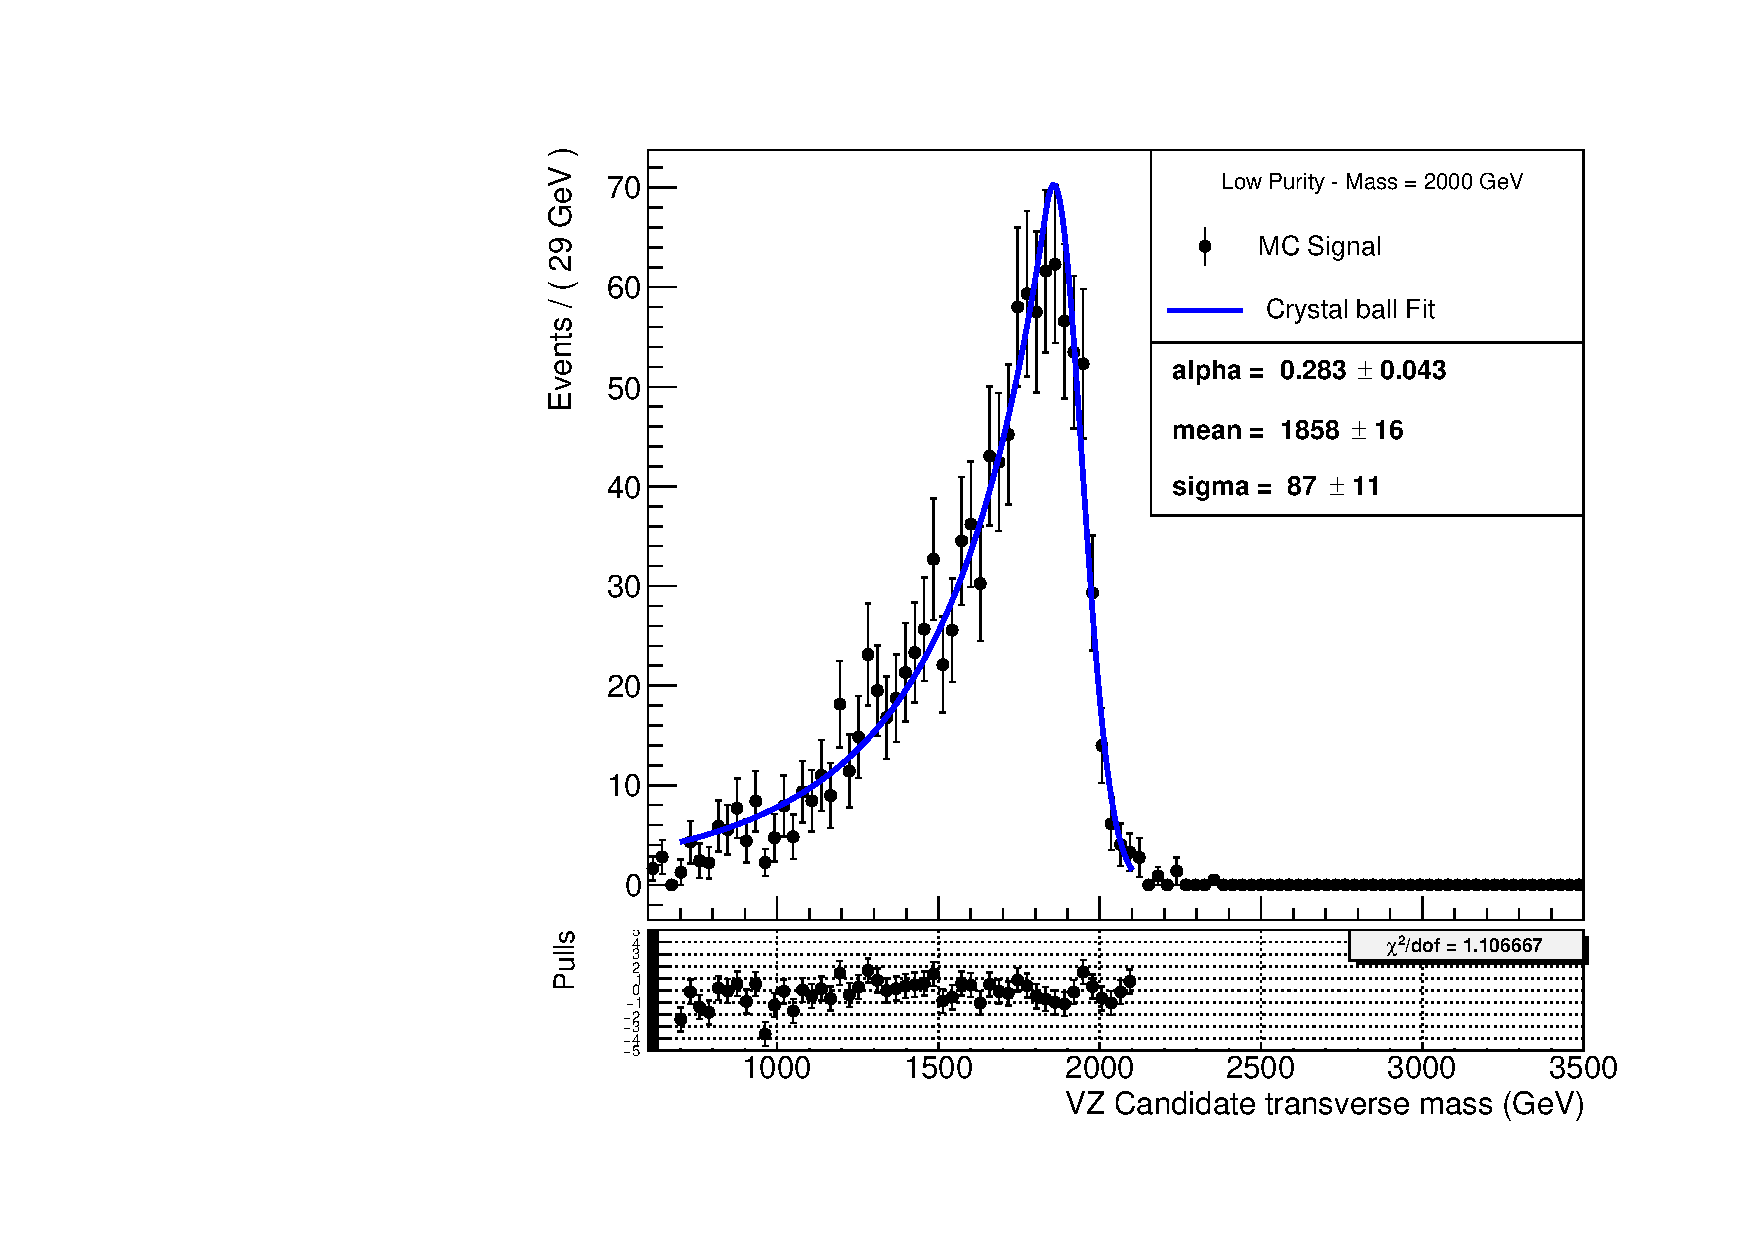
\includegraphics[width=150pt]{figuresARC/fits/WprimeLP2000.pdf}\\
\end{tabular}
\label{fig:fits7}
\end{figure}


\begin{figure}[!ht]
\caption{ Linear interpolation in the Crtsyal-Ball fit model with a step of 100 GeV for bulk graviton samples.}
\begin{center}
  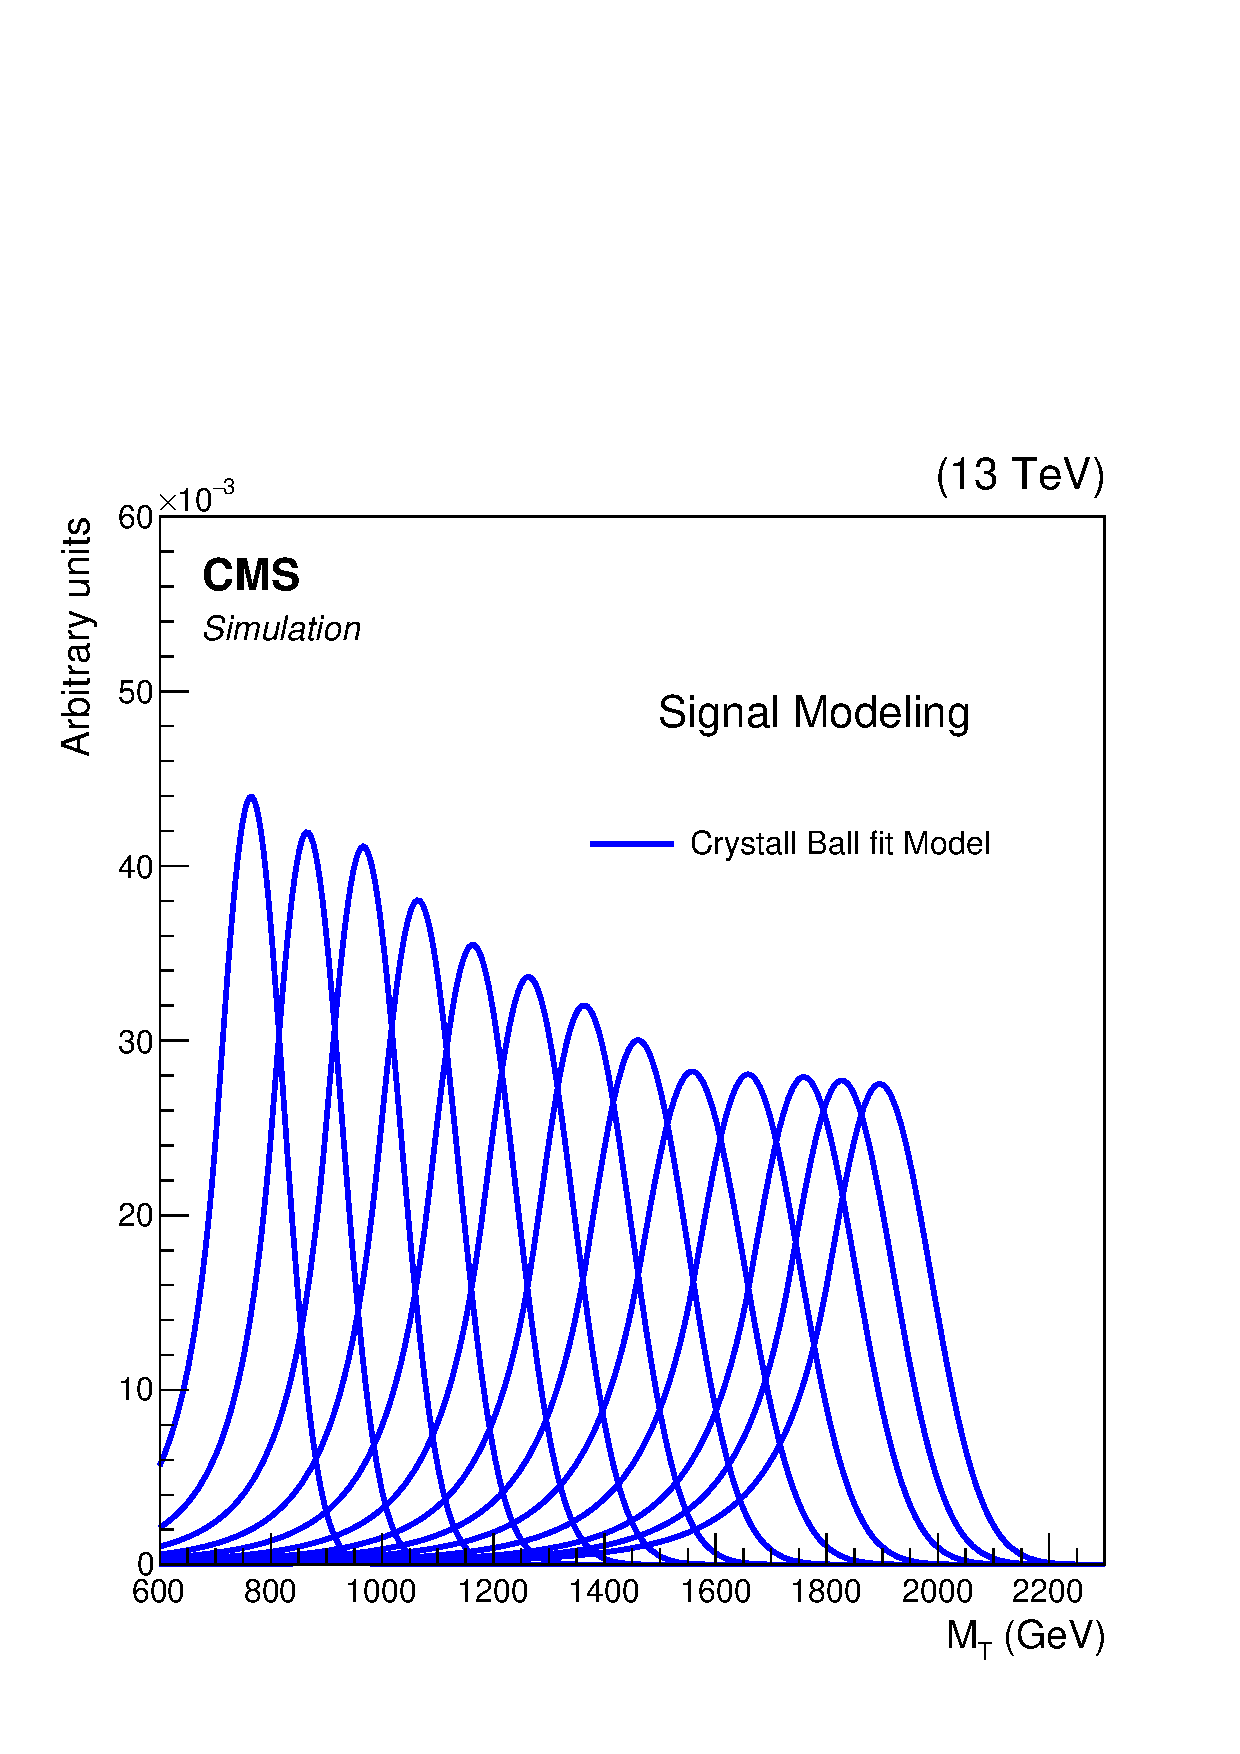
\includegraphics[height=8cm,width=7cm]{figuresARC/fits/testRGS.pdf} 
\end{center}
\label{fig:fits9}
\end{figure}


